\chapter{\ifproject%
\ifenglish Project Structure and Methodology\else โครงสร้างและขั้นตอนการทำงาน\fi
\else%
\ifenglish Project Structure\else โครงสร้างของโครงงาน\fi
\fi
}

ในบทนี้จะกล่าวถึงหลักการ และการออกแบบระบบ โดยการออกแบบเกมได้ใช้ Game Design Template Master Doc \cite{GDD1, GDD2} เป็นต้นแบบ ซึ่งการพัฒนาจะเป็นแบบ iterative process และมีการสร้าง prototype เพื่อทดสอบวิธีการเล่นและกลไกว่าเป็นไปตามที่ต้องการหรือไม่

\makeatletter

% \renewcommand\section{\@startsection {section}{1}{\z@}%
%                                    {13.5ex \@plus -1ex \@minus -.2ex}%
%                                    {2.3ex \@plus.2ex}%
%                                    {\normalfont\large\bfseries}}

\makeatother
%\vspace{2ex}
% \titleformat{\section}{\normalfont\bfseries}{\thesection}{1em}{}
% \titlespacing*{\section}{0pt}{10ex}{0pt}

\section{การรวบรวมความต้องการ (Requirement Gathering)}

ในขั้นตอนนี้ทางทีมผู้พัฒนาได้ไปสำรวจข้อคิดเห็นของผู้เล่นต่อเกมในท้องตลาดถึงสิ่งที่ผู้เล่นรู้สึกว่าเกมสยองขวัญแบบผู้เล่นหลายคนควรทำใด้ดีกว่า โดยได้สำรวจผ่านช่องทางสังคมออนไลน์ เช่น subreddit, Facebook, Youtube

\subsection{สิ่งที่ผู้เล่นต้องการให้ดีขึ้นในเกมสยองขวัญแบบผู้เล่นหลายคน}

\begin{enumerate}
  \item ศัตรูที่คาดเดาได้ยาก เกมสยองขวัญแบบผู้เล่นหลายคน มักจะมีศัตรูที่มีพลังและการเคลื่อนไหวที่หลากหลาย แต่ผู้เล่นสามารถคาดเดาได้ง่าย ผู้เล่นจะรู้สึกว่าเกมนั้นไม่น่าสนใจและไม่มีความสนุก ไม่มีความน่ากลัว
  \item ความยากของเกมที่สมดุลขึ้น ในบางเกมที่ความยากจะมากขึ้นตามความก้าวหน้าของการเล่นจะต้องมีการจัดสมดุลที่ดี ไม่ยากจนเกินไป เกมหนึ่งที่ทำได้ดีคือ Left 4 Dead ซึ่งมี AI ที่เรียกว่า The Director มีหน้าที่ควบคุมการดำเนินไปของการเล่น ความเข้มข้นของเกม จังหวะการโจมตี จำนวนศัตรู การเกิดขึ้นของไอเทม และการเกิดขึ้นของศัตรู ระบบนี้มุ่งเน้นที่ประสบการณ์ของผู้เล่นแต่ละคนเพื่อให้แต่ละคนสามารถเล่นเกมได้อย่างสนุกไม่เบื่อและกลับมาเล่นซ้ำได้โดยที่แต่ละรอบมีความแตกต่างกัน \cite{DirectorL4D}
  \item Replayability mechanism ที่ไม่ผูกกับการต้องกลับมาเล่นซ้ำเพื่อให้เก่งขึ้น การกลับมาเล่นเกมของผู้พัฒนาซ้ำบ่อย ๆ เป็นสิ่งที่ดี แต่ถ้าบังคับผู้เล่นมากเกินไป ผู้เล่นจะรู้สึกว่าตนมีภาระงาน ผู้เล่นไม่ชอบการที่ความสามารถดี ๆ ของตัวละครเข้าถึงได้ยาก ต้องเล่นให้ผ่านเยอะ ๆ อีกทั้งเกมจะสูญเสียความน่ากลัวเพราะการได้เล่นซ้ำเยอะ ๆ ผนวกกับประเด็นที่กล่าวข้างต้น เกมหนึ่งที่ไม่มี Progression mechanism คือ Left 4 Dead \cite{IconicL4D} ซึ่งผู้เล่นสามารถเล่นได้หลายรอบ แต่ผู้เล่นก็ยังรู้สึกว่าเกมนั้นน่ากลัว น่าเล่น และรู้สึกสนุกกับเพื่อน ๆ ได้ The Director ของ Left 4 Dead ทำหน้าที่ให้ประสบการณ์การเล่นแต่ละรอบไม่เหมือนกัน เป็นวิธีเพิ่ม Replayability แบบหนึ่งนอกเหนือจาก Progression
  \item ศัตรูที่เป็นเอกลักษณ์ ศัตรูที่เป็นเอกลักษณ์จะช่วยให้เกมโดดเด่น เป็นที่จดจำของผู้เล่น และช่วยเสริมบรรยากาศให้น่ากลัวมากขึ้น
  \item เนื้อเรื่องที่น่าสนใจ มีเหตุมีผลต่อเหตุการณ์ที่เกิดขึ้นในเกมจะช่วยเสริมความน่ากลัว ทำให้ผู้เล่นสนใจ รู้สึกเหมือนเป็นส่วนหนึ่งของเกมมากขึ้น
\end{enumerate}

% \subsection{เกมที่ประสบความสำเร็จ}

% \subsubsection{Left 4 Dead}

% เกมนี้ถือว่าเป็นเกมสยองขวัญแบบผู้เล่นหลายคนที่โดดเด่นแม้ว่าจะถูกปล่อยออกมาเมื่อกว่า 10 ปีก่อน \\ เหตุผลที่เกมนี้มีผู้เล่นอยู่เรื่อย ๆ เพราะว่าผู้เล่นไม่จำเป็นต้องเรียนรู้เยอะมาก เหมาะกับการชวนเพื่อนใหม่มาเล่นโดยไม่ต้องสอน เกมนี้ไม่มี progression เช่น skill tree หรือ level ที่เรามักเห็นกันในเกมสมัยใหม่ นั่นทำให้ผู้เล่นรู้สึกว่าการเล่นเกมนี้ไม่ได้สร้างข้อบังคับว่าต้องมาเล่นบ่อย ๆ แล้วจะเก่งขึ้น อีกทั้งยังทำให้ช่องว่างระหว่างผู้เล่นที่มีประสบการณ์และผู้เล่นใหม่น้อย ผู้เล่นทั้งสองกลุ่มสามารถร่วมเล่นเกมด้วยกันได้อย่างสนุกสนาน ในด้านทางเทคนิค AI ของเกมมีความล้ำหน้ามากเมื่อ 10 ปีก่อน การหาเส้นทาง (Pathfinding) ของศัตรูมีความหลากหลาย ศัตรูสามารถปีนขึ้นปีนลงบันไดและกำแพงได้ สามารถทำร้ายผู้เล่นแบบลอบเร้นได้อย่างแยบยล เกม Left 4 Dead ยังมี AI ที่เรียกว่า The Director มีหน้าที่ควบคุมการดำเนินไปของการเล่น ความเข้มข้นของเกม จังหวะการโจมตี จำนวนศัตรู การเกิดขึ้นของไอเทม และการเกิดขึ้นของศัตรู ระบบนี้มุ่งเน้นที่ประสบการณ์ของผู้เล่นแต่ละคนเพื่อให้แต่ละคนสามารถเล่นเกมได้อย่างสนุกไม่เบื่อและกลับมาเล่นซ้ำได้โดยที่แต่ละรอบมีความแตกต่างกัน

% ทางทีมพัฒนาได้ลองเล่นเกมนี้แล้วพบว่าเกมนี้มีเป็นเกมที่ไม่ต้องเรียนรู้เยอะ สนุก สามารถเล่นได้เมื่อไรก็ได้ มีเนื้อหาเยอะ แต่ละรอบที่เล่นมีความแตกต่างกันจริงขึ้นอยู่กับฝีมือการเล่นในแต่ละรอบ

\section{ภาพรวมของเกม (Summary)}

ใน Two-player Cooperative Horror Game ผู้เล่นรับบทเป็นนายพรานและแม่ชี มีหน้าที่ช่วยกันปราบปีศาจร้ายในป่า โดยต้องทำภารกิจทำลายวงแหวนเวทย์ที่กระจัดกระจายอยู่รอบป่า พร้อมทั้งเอาตัวรอดจากปีศาจ ซึ่งปีศาจแปลงกลายเป็นสัตว์ แฝงตัวอยู่ในฝูงของสัตว์อื่น ๆ  ผู้เล่นทั้งสองจะมีหน้าที่และความสามารถที่แตกต่างกัน ทั้งคู่ต้องช่วยกันถึงจะสามารถปราบปีศาจนี้ได้

\section{แนวคิดหลักของเกม (Core)}

\subsection{Design Pillars}

เป็นรากฐานของเกมที่จะไม่เปลี่ยนแปลง และการออกแบบส่วนต่าง ๆ ของเกมควรสอดรับกับสิ่งเหล่านี้ \cite{GDD1}

\begin{enumerate}
  \item เกมสยองขวัญที่ผู้เล่นต้องช่วยกันถึงจะผ่านไปได้
  \item ผู้เล่นแต่ละคนมีความสามารถแตกต่างกัน ต้องทำงานร่วมกันถึงจะสำเร็จ
  \item เกมมีความท้าทายในทุกครั้งที่เล่น สามารถเล่นซ้ำได้โดยไม่รู้สึกเบื่อ
\end{enumerate}

\subsection{Game Loops}

ผู้เล่นทั้งสองต้องช่วยกันทำลายวงแหวนเวทย์มนต์ตามที่ต่าง ๆ พร้อมเอาชีวิตรอดจากปีศาจ

\subsection{แรงจูงใจในการเล่น (Player Motivation)}

ผู้เล่นมีแรงจูงใจในการเล่นเพื่อเอาชนะปีศาจ และเมื่อเล่นต่อไปหลังจากจบหนึ่งเกมหรือขณะเล่นอยู่ เกมจะยากขึ้นและบีบให้ผู้เล่นเล่นในแบบที่ยังไม่เคยเล่นมาก่อน ผู้เล่นมีแรงจูงใจในการเล่นมากขึ้นมื่อเล่นกับเพื่อน

\section{เนื้อหา}

\subsection{โดยรวม}

เกมนี้เป็นเกมสยองขวัญที่อาศัยความร่วมมือของผู้เล่นสองคน เป็นเกมมุมมองบุคคลที่หนึ่ง งานภาพเป็นแนว 3D Photorealistic หนึ่งเกมสามารถเล่นจบภายในเวลา 30-40 นาที

\subsection{เนื้อเรื่อง}

เกมนี้มีเนื่อเรื่องและสถานที่อยู่ในยุโรปยุคกลาง ตามความเชื่อที่ว่า ปีศาจสามารถปลอมแปลงเป็นสัตว์ชนิดหนึ่ง อาศัยอยู่ในป่ารกร้าง หน้าที่ของผู้เล่นคือ ต้องไปปราบปีศาจร้ายและทำให้ผู้คนปลอดภัย

\subsection{ตัวละคร}

ผู้เล่นสามารถเลือกเล่นเป็นแม่ชี (Nun) หรือนายพราน (Hunter) ซึ่งแต่ละตัวละครมีความสามารถแตกต่างกันไป

\subsubsection{ตัวละครนายพราน (Hunter)}

\paragraph{ความสามารถ}
\begin{itemize}
  \item สามารถปกป้องแม่ชีจากกับดักในป่าได้
  \item สามารถรักษาตัวเองและแม่ชี โดยใช้สมุนไพรในป่า
  \item มีแผนที่ใช้นำทาง สามารถทำเครื่องหมายบนแผนที่ได้
\end{itemize}

\paragraph{การออกแบบ}
\begin{itemize}
  \item เป็นชาวยุโรปผิวขาว
  \item มีหนวดเคราและผมสีดำยาว
  \item อายุประมาณ 40 ปี
  \item สวมชุดนายพราน
\end{itemize}

\subsubsection{ตัวละครแม่ชี (Nun)}

\paragraph{ความสามารถ}
\begin{itemize}
  \item สามารถป้องกันการโจมตีจากปีศาจ
  \item สามารถทำลายวงแหวนเวทย์มนต์ได้
  \item มีสายตาที่แย่ไม่สามารถเห็นได้ในระยะไกล
  \item แต่สามารถเห็นปีศาจในระยะไกล และรู้ว่าปีศาจคือสัตว์ตัวไหน
  \item สามารถรับรู้ได้ถึงวงแหวนเวทย์มนต์จากระยะไกล
\end{itemize}

\paragraph{การออกแบบ}
\begin{itemize}
  \item เป็นชาวยุโรปผิวขาว
  \item สวมชุดแม่ชี
  \item อายุประมาณ 35 ปี
\end{itemize}

\subsubsection{ปีศาจ}

ปีศาจเป็นสัตว์หน้าตาดูปกติ อาศัยอยู่ในป่า แฝงตัวอยู่ตามฝูงสัตว์ปกติอื่น ๆ สัตว์ที่เป็นปีศาจได้ ประกอบไปด้วย
\begin{itemize}
  \item สุนัขจิ้งจอก
  \item หมาป่า
  \item กวางตัวผู้
  \item กวางตัวเมีย
\end{itemize}

การที่ปีศาจหน้าตาดูปกติและนายพรานไม่สามารถรู้ได้ว่าสัตว์ตัวไหนเป็นตัวร้ายท่ามกลางสัตว์ปกติในเกม ทำให้ต้องมีการสื่อสารกันระหว่างผู้เล่น ทำให้เกิดอารมณ์ระแวง เพิ่มความตึงเครียด และความท้าทายให้กับเกม

\begin{figure}[h]
  \centering
  \begin{subfigure}{0.4\textwidth}
    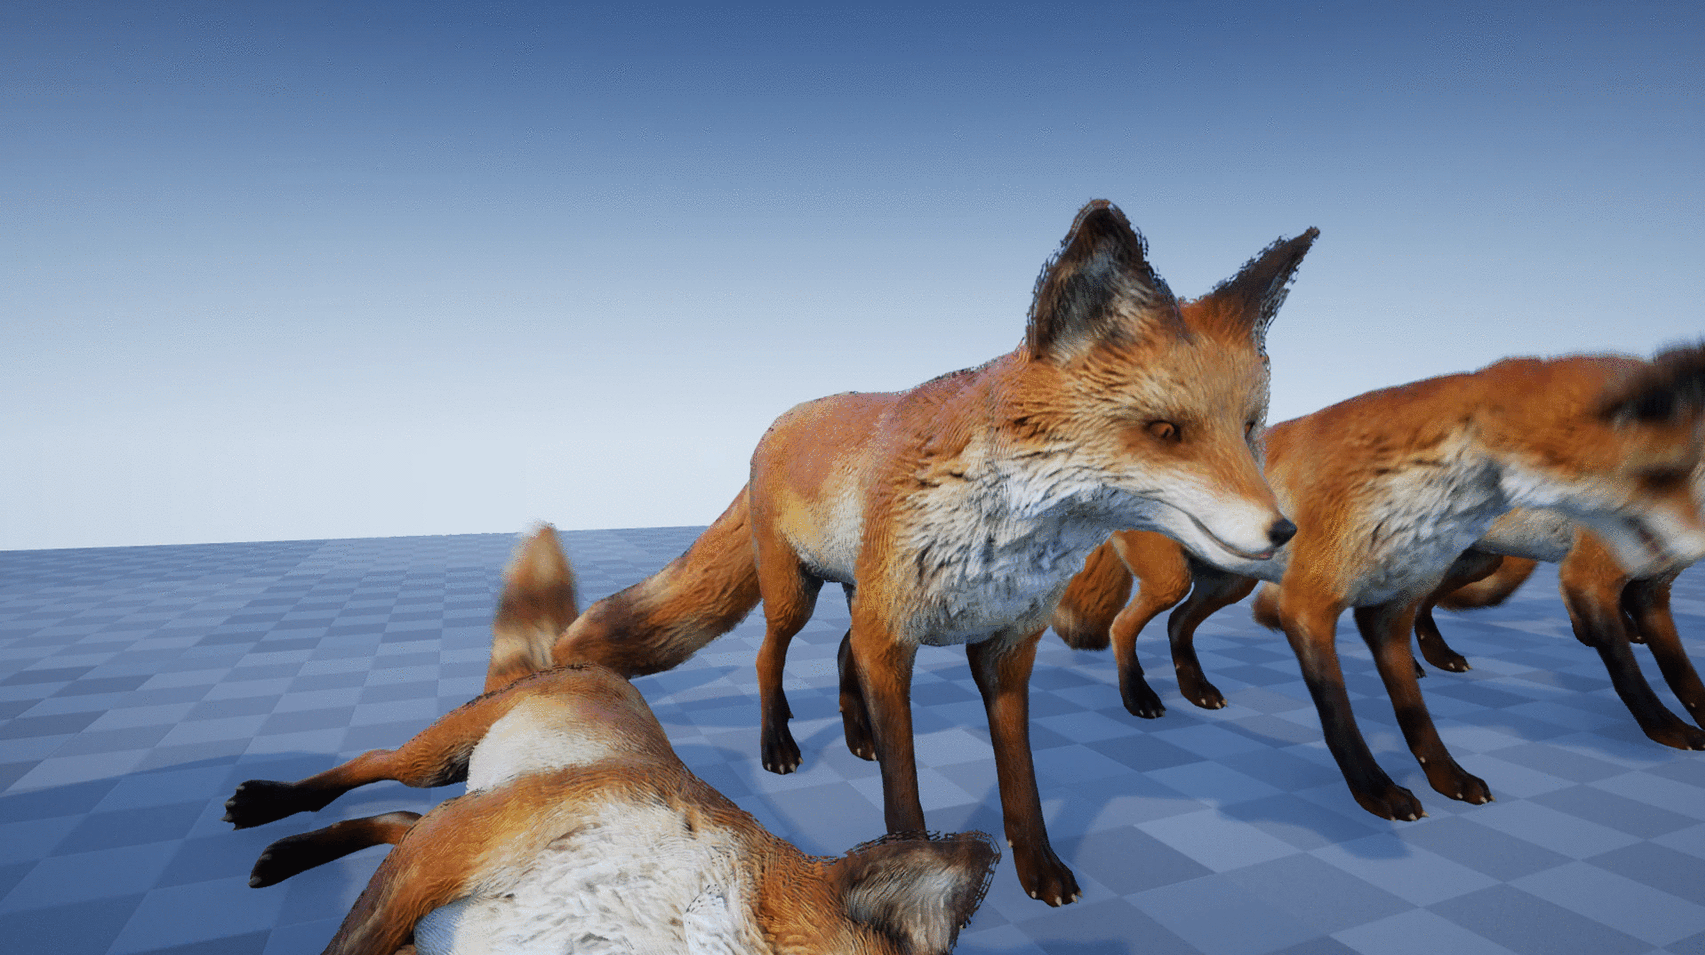
\includegraphics[width=\textwidth]{./img/fox.png}
    \caption[สุนัขจิ้งจอกในเกม]{สุนัขจิ้งจอกในเกม}
    \label{fig:fox}
  \end{subfigure}
  \hfil
  \begin{subfigure}{0.4\textwidth}
    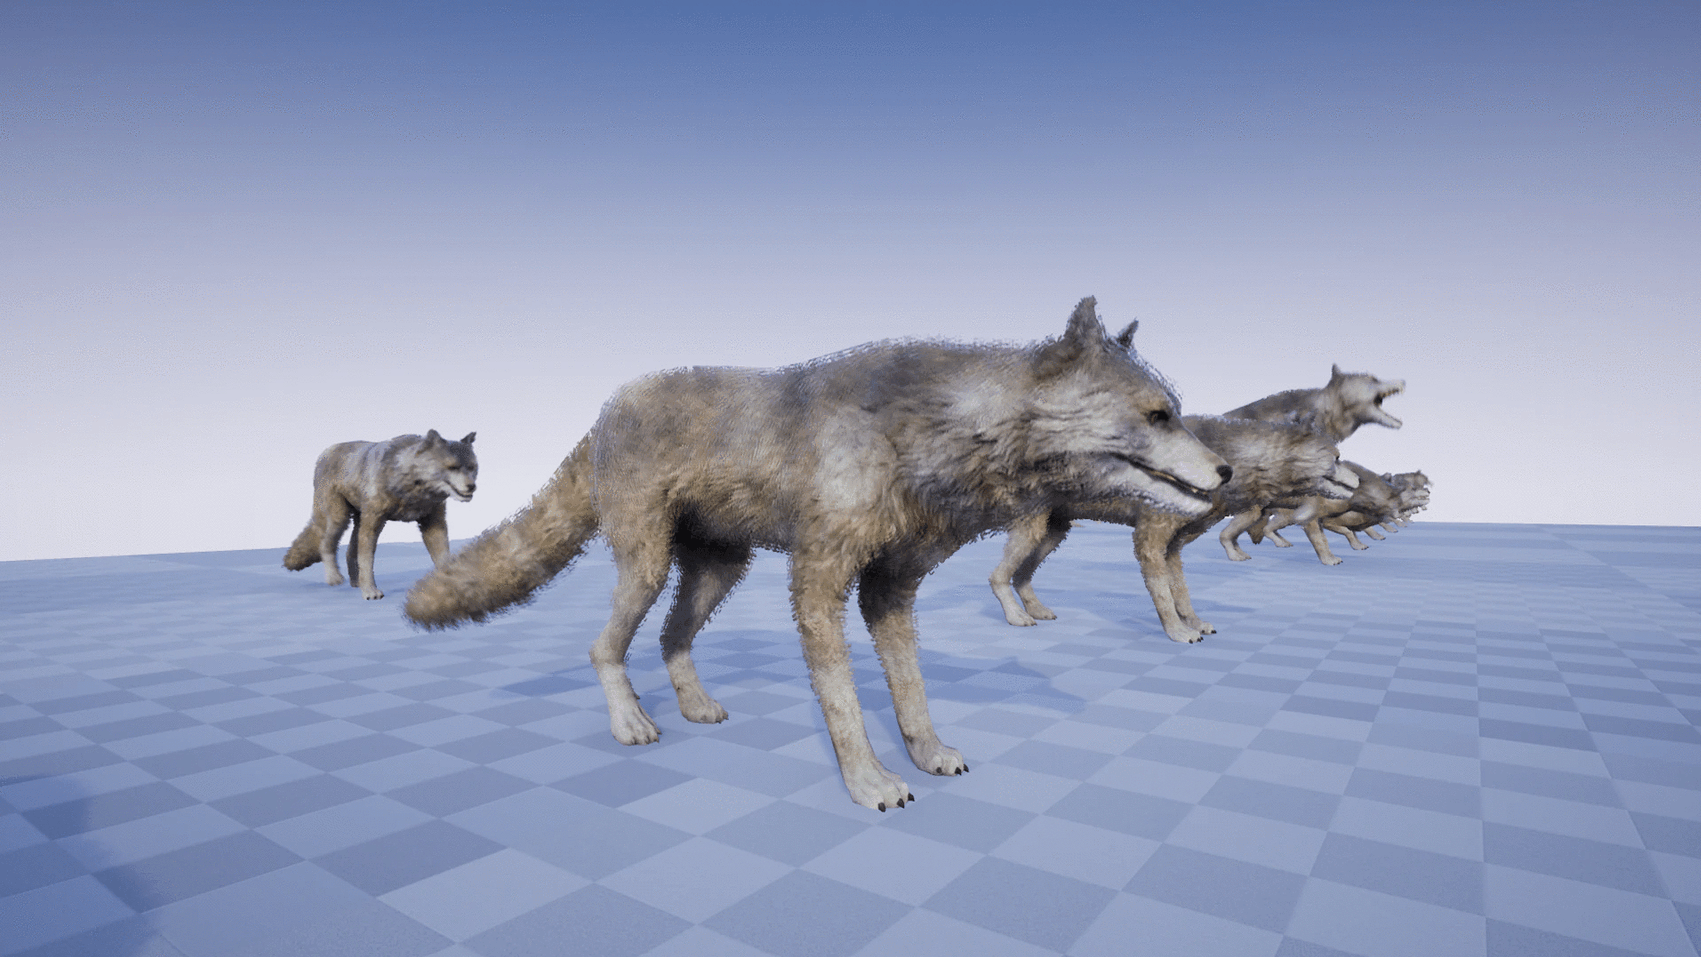
\includegraphics[width=\textwidth]{./img/wolf.png}
    \caption[หมาป่าในเกม]{หมาป่าในเกม}
    \label{fig:wolf}
  \end{subfigure}
  \hfil
  \begin{subfigure}{0.4\textwidth}
    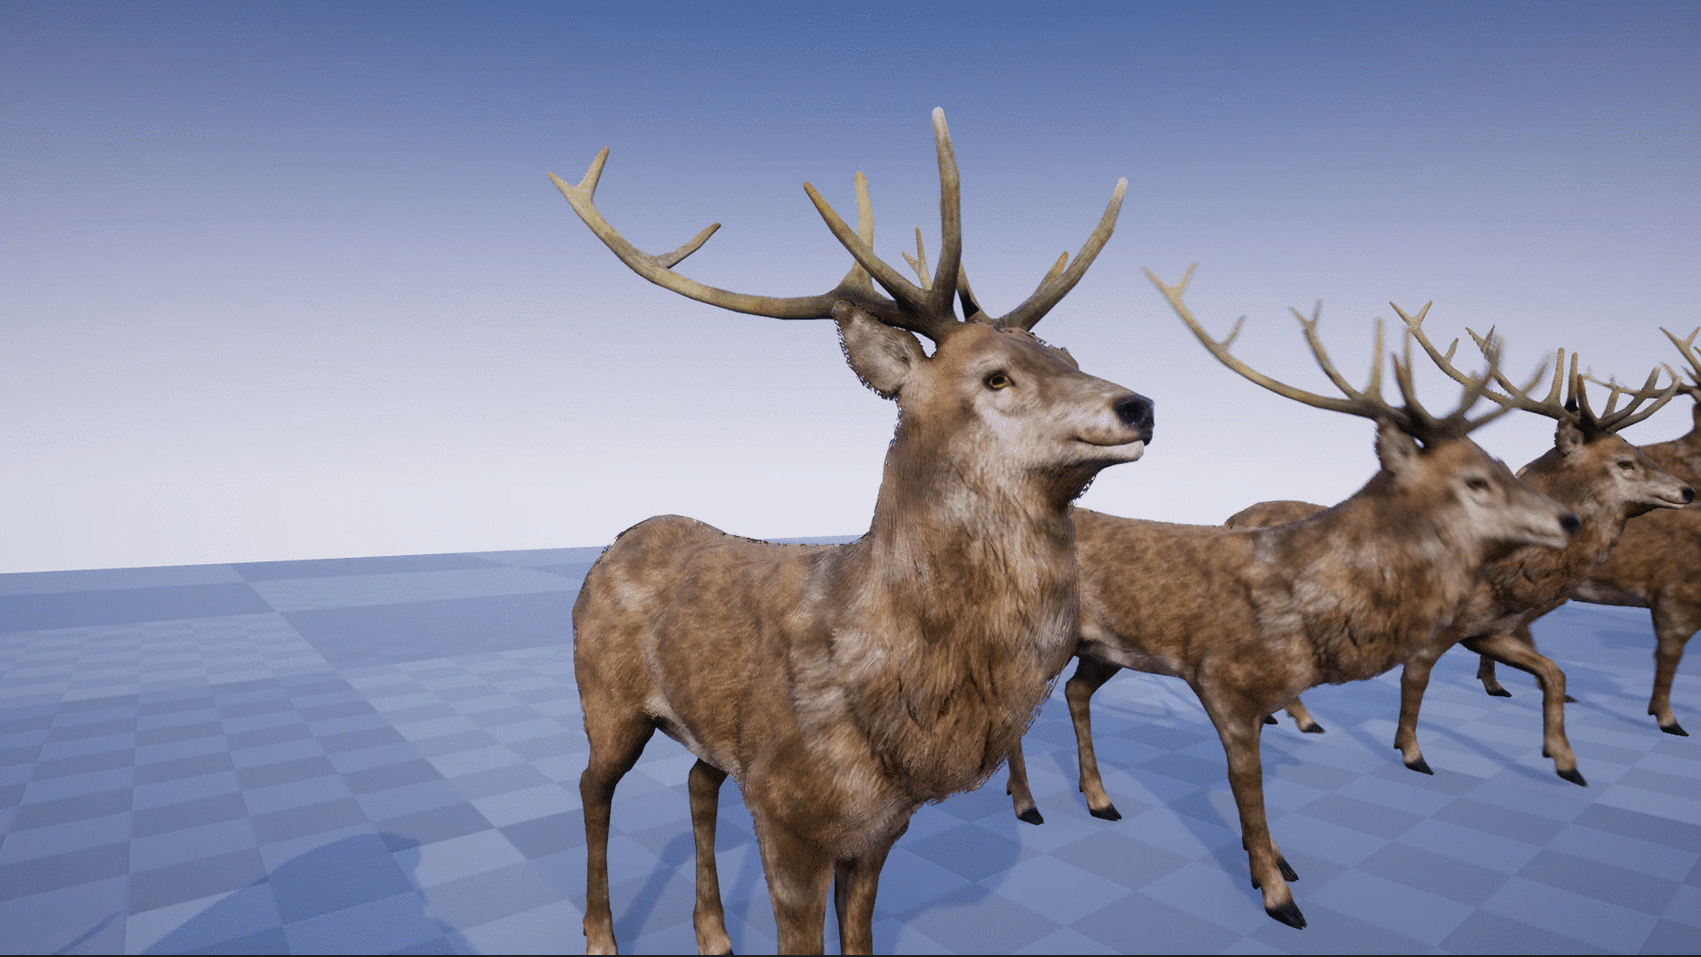
\includegraphics[width=\textwidth]{./img/deerstag.png}
    \caption[กวางตัวผู้ในเกม]{กวางตัวผู้ในเกม}
    \label{fig:deerstag}
  \end{subfigure}
  \hfil
  \begin{subfigure}{0.4\textwidth}
    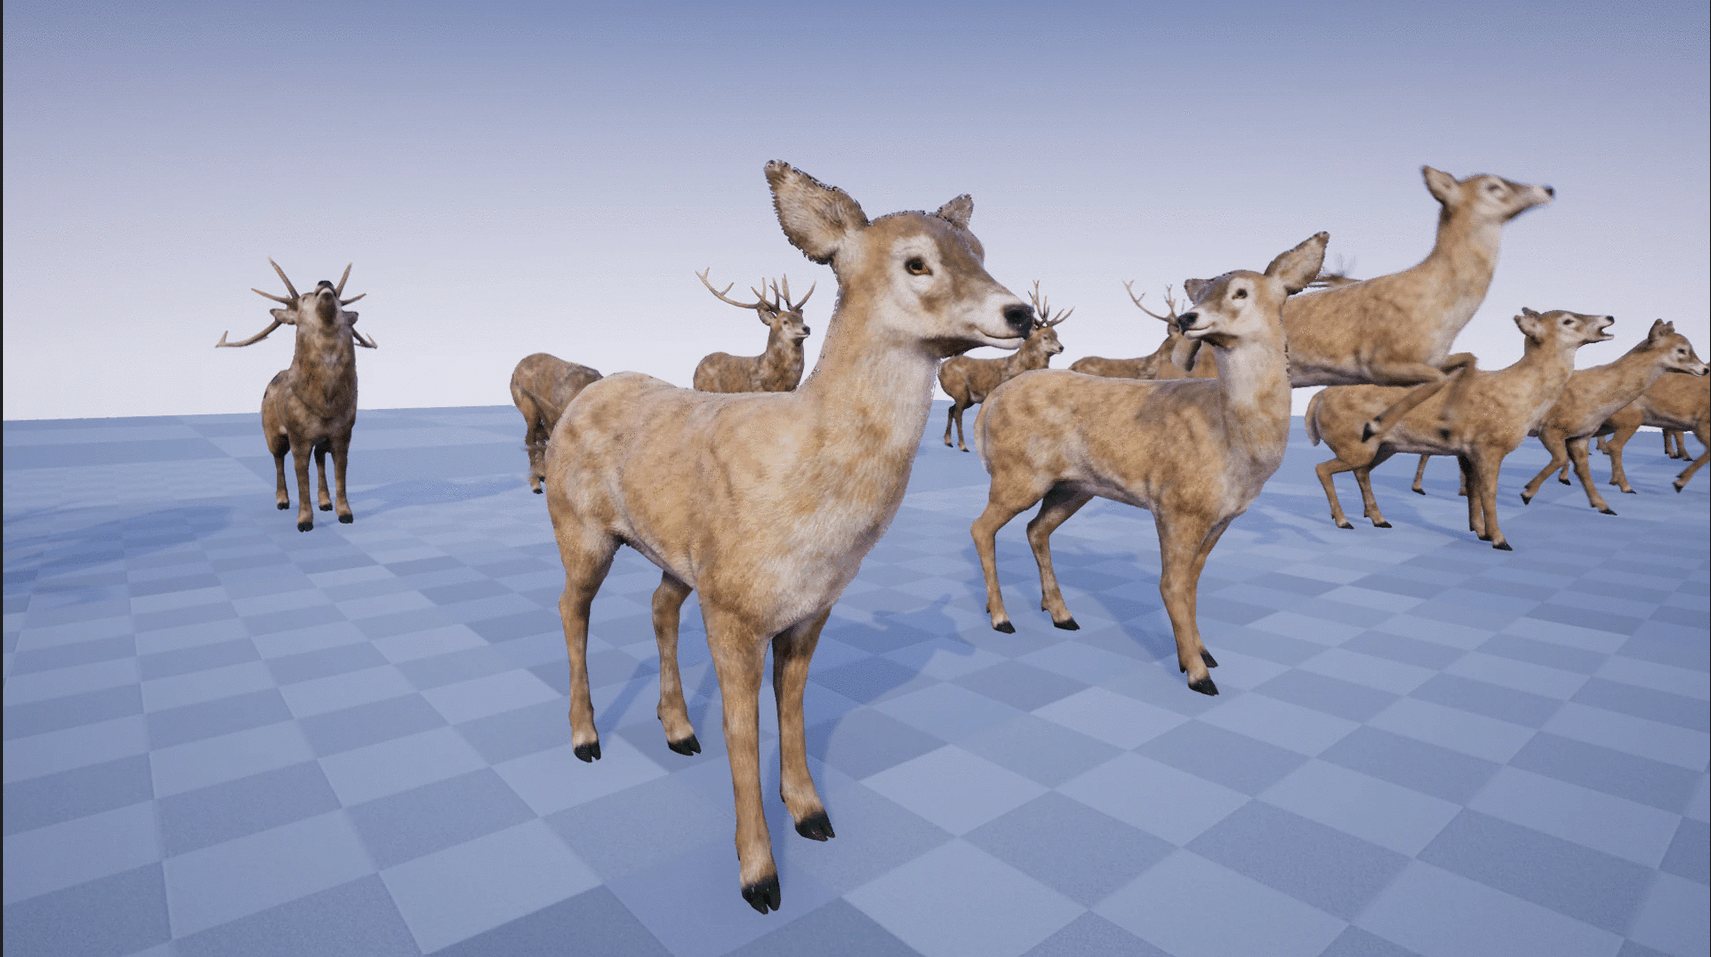
\includegraphics[width=\textwidth]{./img/deerdoe.png}
    \caption[กวางตัวเมียในเกม]{กวางตัวเมียในเกม}
    \label{fig:deerdoe}
  \end{subfigure}
  \caption{รูปสัตว์ในเกมซึ่งเป็นปีศาจ}
  \label{fig:four animals}
\end{figure}

% \begin{figure}[h]
%   \begin{center}
%   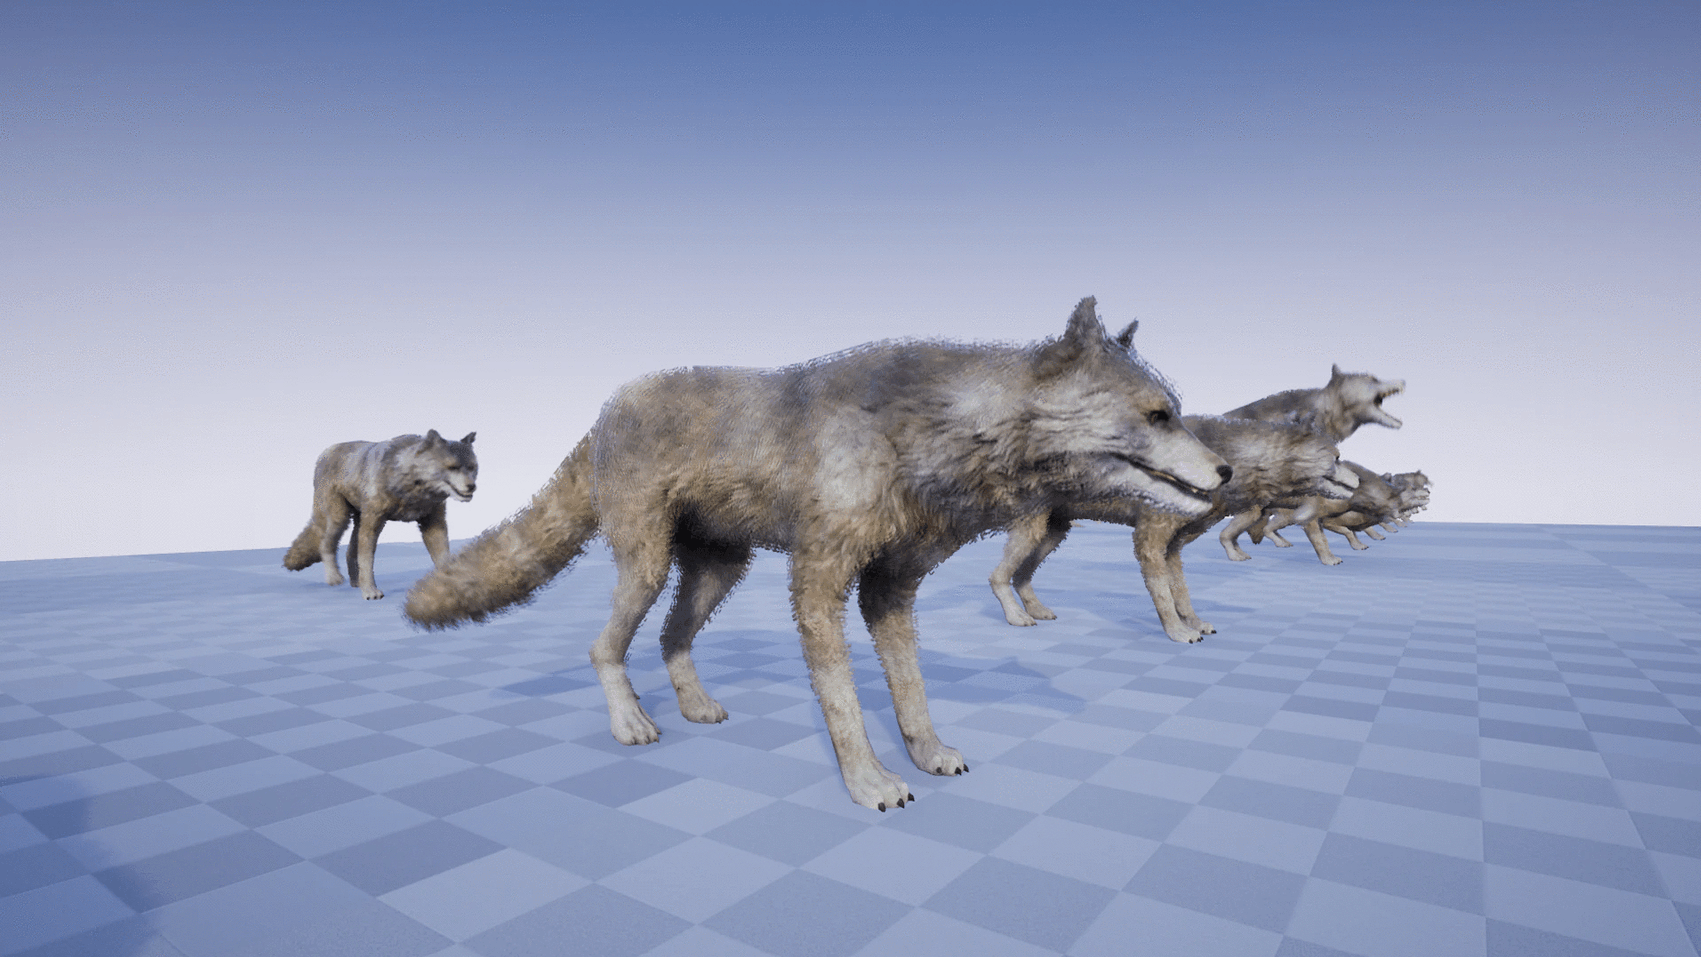
\includegraphics[width=\textwidth]{./img/wolf.png}
%   \end{center}
%   \caption[หมาป่าในเกม]{หมาป่าในเกม}
%   \label{fig:wolf}
% \end{figure}

% \begin{figure}[h]
%   \begin{center}
%   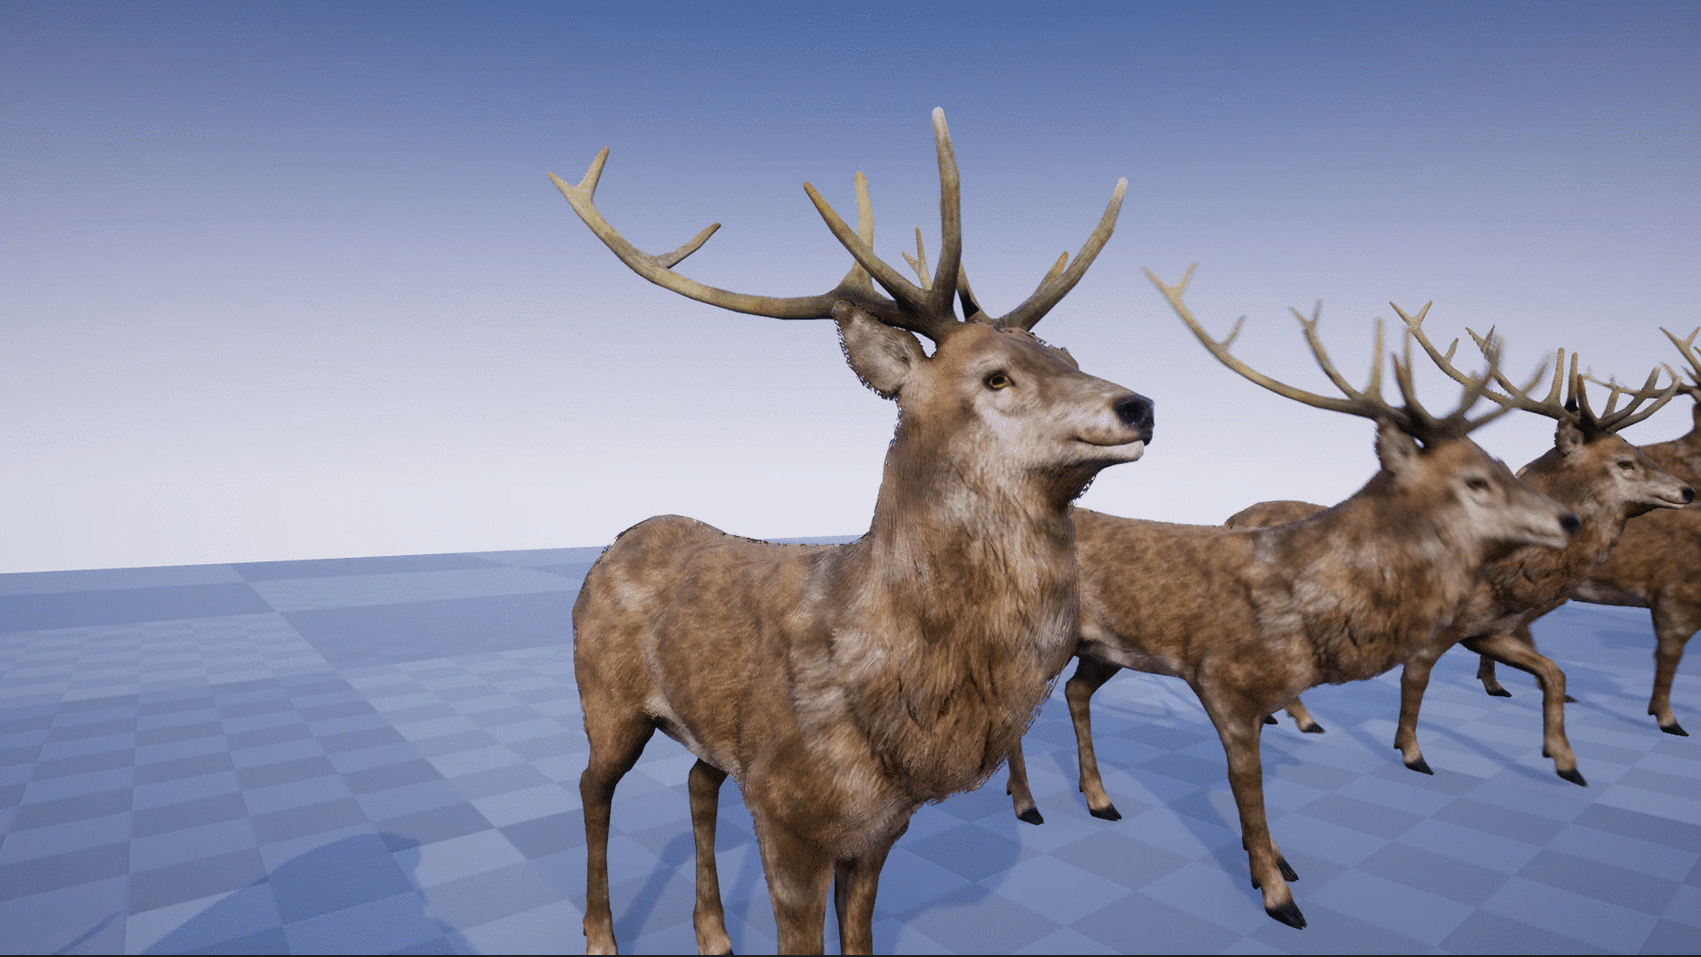
\includegraphics[width=\textwidth]{./img/deerstag.png}
%   \end{center}
%   \caption[กวางตัวผู้ในเกม]{กวางตัวผู้ในเกม}
%   \label{fig:deerstag}
% \end{figure}

% \begin{figure}[h]
%   \begin{center}
%   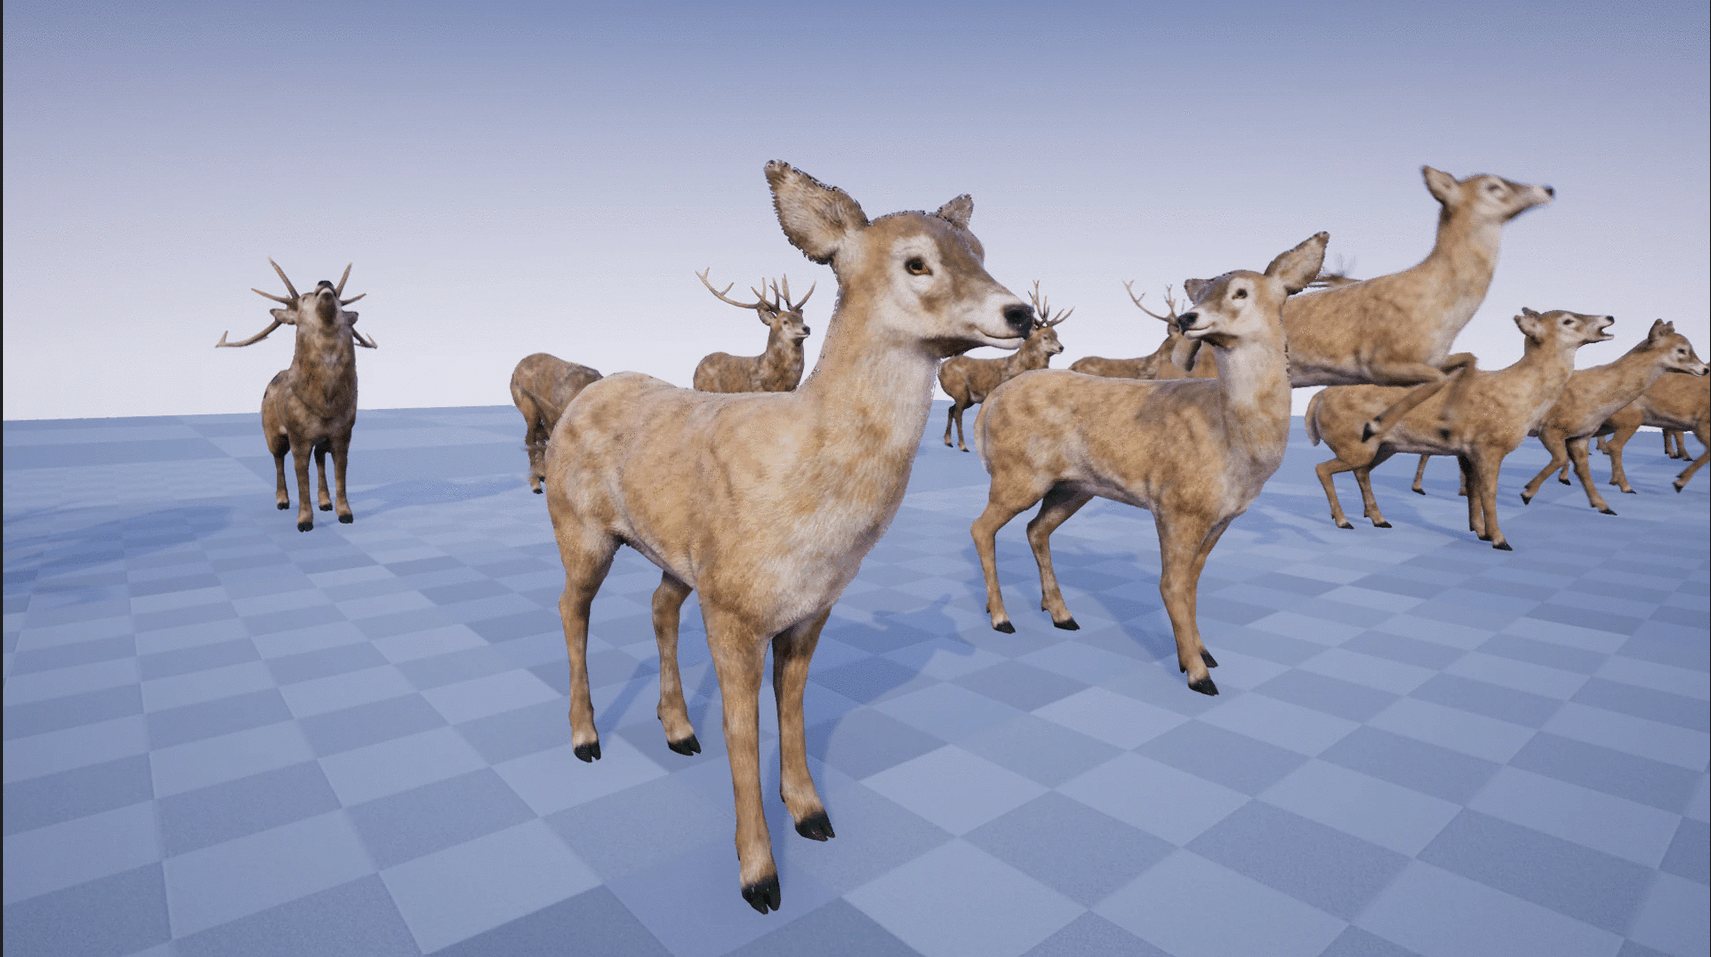
\includegraphics[width=\textwidth]{./img/deerdoe.png}
%   \end{center}
%   \caption[กวางตัวเมียในเกม]{กวางตัวเมียในเกม}
%   \label{fig:deerdoe}
% \end{figure}

\subsection{ฉาก}

สถานที่ของเกม คือ ป่ารกร้างในยุโรปยุคกลาง ต้นไม้ในฉากจะไม่มีใบหรือใบแห้งแร้งมาก บนพื้นจะเต็มไปด้วยหญ้าแห้งและใบไม้แห้ง ให้อารมณ์ความรู้สึกที่โดดเดี่ยว ไร้ชีวิตชีวา ทั้งในยามกลางวันและกลางคืน ต้นไม้ประกอบฉากต้องเป็นต้นไม้ในป่ายุโรป เช่น European Hornbeam, Black Alder, ฺBeech Tree ภูมิประเทศเป็นพื้นที่ราบมีเนินและแหล่งน้ำบ้าง เพื่อเพิ่มความน่าสนใจและมีจุดสังเกตุให้ผู้เล่น

ฉากของเกมควรมีขนาดที่ใหญ่เหมาะสมที่ให้ผู้เล่นสามารถสำรวจสถานที่ทั้งหมดได้ภายในเวลาไม่เกิน 20 นาที จากระยะเวลาการเล่นทั้งหมด 30-40 นาที

\begin{figure}[h]
  \begin{center}
  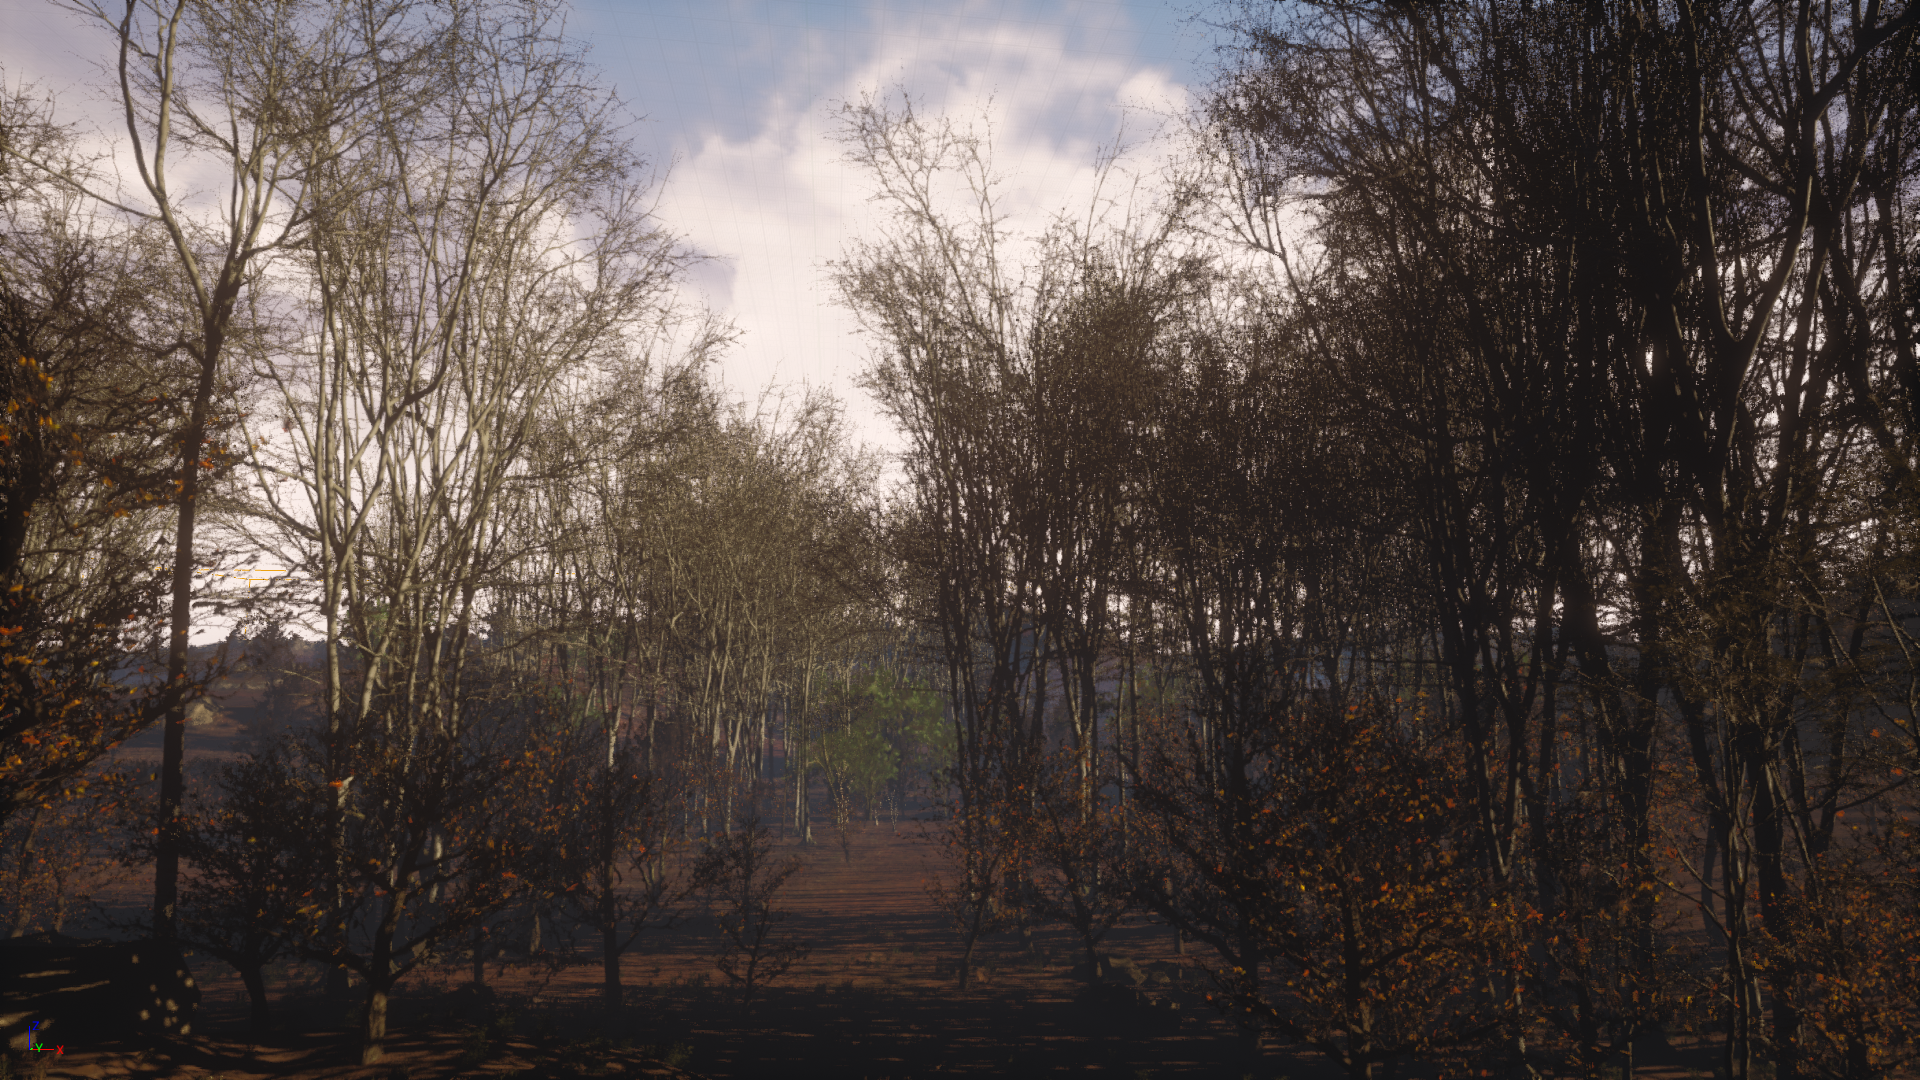
\includegraphics[width=\textwidth]{./img/screenshots/dayshot2.png}
  \end{center}
  \caption[ภาพฉากใน Two-player Cooperative Horror Game]{ภาพฉากใน Two-player Cooperative Horror Game}
  \label{fig:gameshot}
\end{figure}
\subsection{เสียงและดนตรีประกอบ}

ดนตรีประกอบเป็นดนตรีตะวันตก ใช้เครื่องดนตรียุโรปยุคกลางผสมสมัยคลาสสิค จะต้องมีดนตรีในช่วงที่ต่อสู้กับปีศาจ ช่วงที่กำลังทำลายวงแหวนเวทย์มนต์ และช่วงสำคัญอื่น ๆ โดยรวมแล้วดนตรีประกอบต้องมีอารมณ์ที่ลุ้นระทึก แต่ไม่ทำลายบรรยากาศที่เหงา น่ากลัว ของเกม อาจมีเสียงดนตรีอื่นที่ใช้สร้างบรรยากาศ เช่น เสียงดนตรี Drone เสียงโน้ตเปียโนที่เล่นแบบย้อนกลับ เป็นต้น

เสียงประกอบที่จำเป็นต้องมี คือ เสียงเดินของตัวละคร เสียงวิ่งของตัวละคร เสียงหอบของผู้เล่น
เสียงเจ็บและตายของตัวละคร เสียงร้องของสัตว์

\section{คุณสมบัติ (Features)}

\subsection{การสร้างฉากที่แตกต่างกัน}

\subsubsection{บริบท (Context)}

คุณสมบัตินี้จำเป็นต้องมีเพื่อให้การเล่นแต่ละครั้งไม่เหมือนกัน เพิ่มความท้าทายและความยากในการเล่นแต่ \\ ละรอบ และเพื่อให้ผู้เล่นสามารถเล่นซ้ำได้โดยไม่รู้สึกเบื่อ

\subsubsection{สมมติฐาน (Hypothesis)}

การสร้างฉากที่แตกต่างกันจะทำให้การเล่นแต่ละครั้งไม่เหมือนกัน สามารถทำให้ผู้เล่นได้เล่นในแบบที่ยังไม่เคยเล่น ทำให้เกมมีความท้าทายในทุกครั้งที่เล่น สามารถเล่นซ้ำได้โดยไม่รู้สึกเบื่อ สัมพันธ์กับ Design Pillar ที่ 3

\subsubsection{วัดผลความสำเร็จ (Measuring success)}

วัดผลโดยความหลากหลายของฉากที่สร้างขึ้น และความยากในการเล่นแต่ละครั้ง ความหลากหลาย เช่น การวางตำแหน่งของไอเทมรู้สึกไม่ซ้ำกัน ความยาก เช่น การสร้างฉากในเกมหน้า ๆ ทำให้รู้สึกว่าเกมยาก แต่เมื่อเล่นจริง ๆ ก็ไม่ยากเท่าที่คิด สามารถเล่นผ่านไปได้ ไม่น่าเบื่อ และยังสนุกอยู่

\subsubsection{การออกแบบ (Design)}

การสร้างฉากในการเล่นแต่ละครั้ง จะเปลี่ยนตำแหน่งและจำนวนของสมุนไพร ตำแหน่งของกับดัก และตำแหน่งของวงแหวนเวทย์มนต์ รวมถึงในการเล่นแต่ละครั้ง ปีศาจจะอยู่ในร่างสัตว์ที่ไม่เหมือนกัน ทั้งนี้การจัดวางสิ่งของต้องมีความสมดุล มีจำนวนที่เหมาะสมที่สามารถเล่นผ่านไปได้อย่างสนุก ไม่ควรกองกันอยู่ที่เดียวกันเยอะเกินไปเพราะจะทำให้เกมจบเร็วขึ้น ไม่สนุก การเปลี่ยนตำแหน่งและจำนวนของสิ่งของจะเพิ่มความท้าทาย และความยากในการเล่นแต่ละรอบได้ในแบบที่ไม่ซ้ำกัน  

\subsection{กลางวันและกลางคืน}

\subsubsection{บริบท (Context)}

คุณสมบัตินี้จำเป็นต้องมีเพื่อให้ผู้เล่นมีโอกาสได้สำรวจพื้นทีและวางแผนอย่างสะดวกตอนกลางวันและเอาชีวิตรอดตอนกลางคืน

\subsubsection{สมมติฐาน (Hypothesis)}

การสร้างกลางวันและกลางคืนจะทำให้ผู้เล่นสามารถสำรวจพื้นที่ได้อย่างสะดวก ผู้เล่นจะสามารถวางแผนการเล่นได้ ทำให้มีแนวทางการเล่นที่หลากหลาย และสามารถเล่นซ้ำได้โดยไม่รู้สึกเบื่อ สัมพันธ์กับ Design Pillar ที่ 3

\subsubsection{วัดผลความสำเร็จ (Measuring success)}

ผู้เล่นสามารถใช้เวลาตอนกลางวันในกาวางแผนและสำรวจพื้นที่ได้ เพื่อให้การเล่นตอนกลางคืนมีความง่ายมากขึ้น ไม่หลงทางตอนกลางคืน สามารถมุ่งเป้าไปที่การสู้กับปีศาจและทำภารกิจได้อย่างสนุก

\subsubsection{การออกแบบ (Design)}

ช่วงเวลากลางวันจะเป็นช่วงเย็น ตอนกลางวันผู้เล่นจะไม่สามารถรู้ว่าปีศาจคือสัตว์ตัวไหน แต่ปีศาจสามารถปรากฏตัวได้อยู่ วงแหวนเวทย์จะยังไม่ปรากฏ ช่วงกลางวันมีไว้เพื่อให้ผู้เล่นสำรวจสถานที่ที่น่าสนใจและเก็บรวบรวมยา สามารถใช้โอกาสนี้สังเกตุสัตว์ที่อยู่ในป่า ปลดกับดัก และทำสัญลักษณของจุดที่สนใจในแผนที่

ช่วงเวลากลางคืนเป็นช่วงที่ปีศาจสามารถทำร้ายเราได้ วงแหวนเวทย์มนต์จะปรากฏขึ้น ผู้เล่นต้องทำหน้าที่ช่วยกันทำลายวงแหวนเวทย์และเอาตัวรอดจากปีศาจ ช่วงนี้จะเป็นช่วงสุดท้ายของเกม (Climax)

ทั้งสองช่วงจะมีการเปลี่ยนผ่านที่เหมือนกับโลกจริง คือ ดวงอาทิตย์เคลื่อนที่ลาลับขอบฟ้า ทั้งสองช่วงกินเวลาเท่ากัน คือ 20 นาที

\subsection{ตะเกียงนำทางในช่วงกลางคืน}
\subsubsection{บริบท (Context)}

คุณสมบัตินี้จำเป็นต้องมีเพราะทำให้ผู้เล่นสามารถเดินทางในช่วงกลางคืนได้อย่างสะดวก

\subsubsection{สมมติฐาน (Hypothesis)}

การเดินทางในช่วงกลางคืนโดนมีตะเกียงจะทำให้ผู้เล่นสามารถเดินทางไปยังสถานที่ที่ต้องการได้อย่างสะดวก แต่อาจใช้เวลาในการเดินทางนานกว่าในช่วงกลางวันเพราะต้องระวังกับดักและปีศาจซึ่งอาจมองไม่เห็นได้ดีเท่าตอนกลางวัน สัมพันธ์กับ Design Pillar ที่ 1

\subsubsection{วัดผลความสำเร็จ}

ผู้เล่นสามารถเดินทางไปยังสถานที่ที่ต้องการได้อย่างสะดวกในตอนกลางคืน

\subsubsection{การออกแบบ}

ผู้เล่นทั้งสองสามารถเปิด ปิดตะเกียงได้ ตะเกียงให้แสงสว่างได้ทั้งเกม ปีศาจจะเห็นผู้เล่นได้ง่ายขึ้นเมื่อเปิดตะเกียง

\begin{figure}[h]
  \begin{center}
  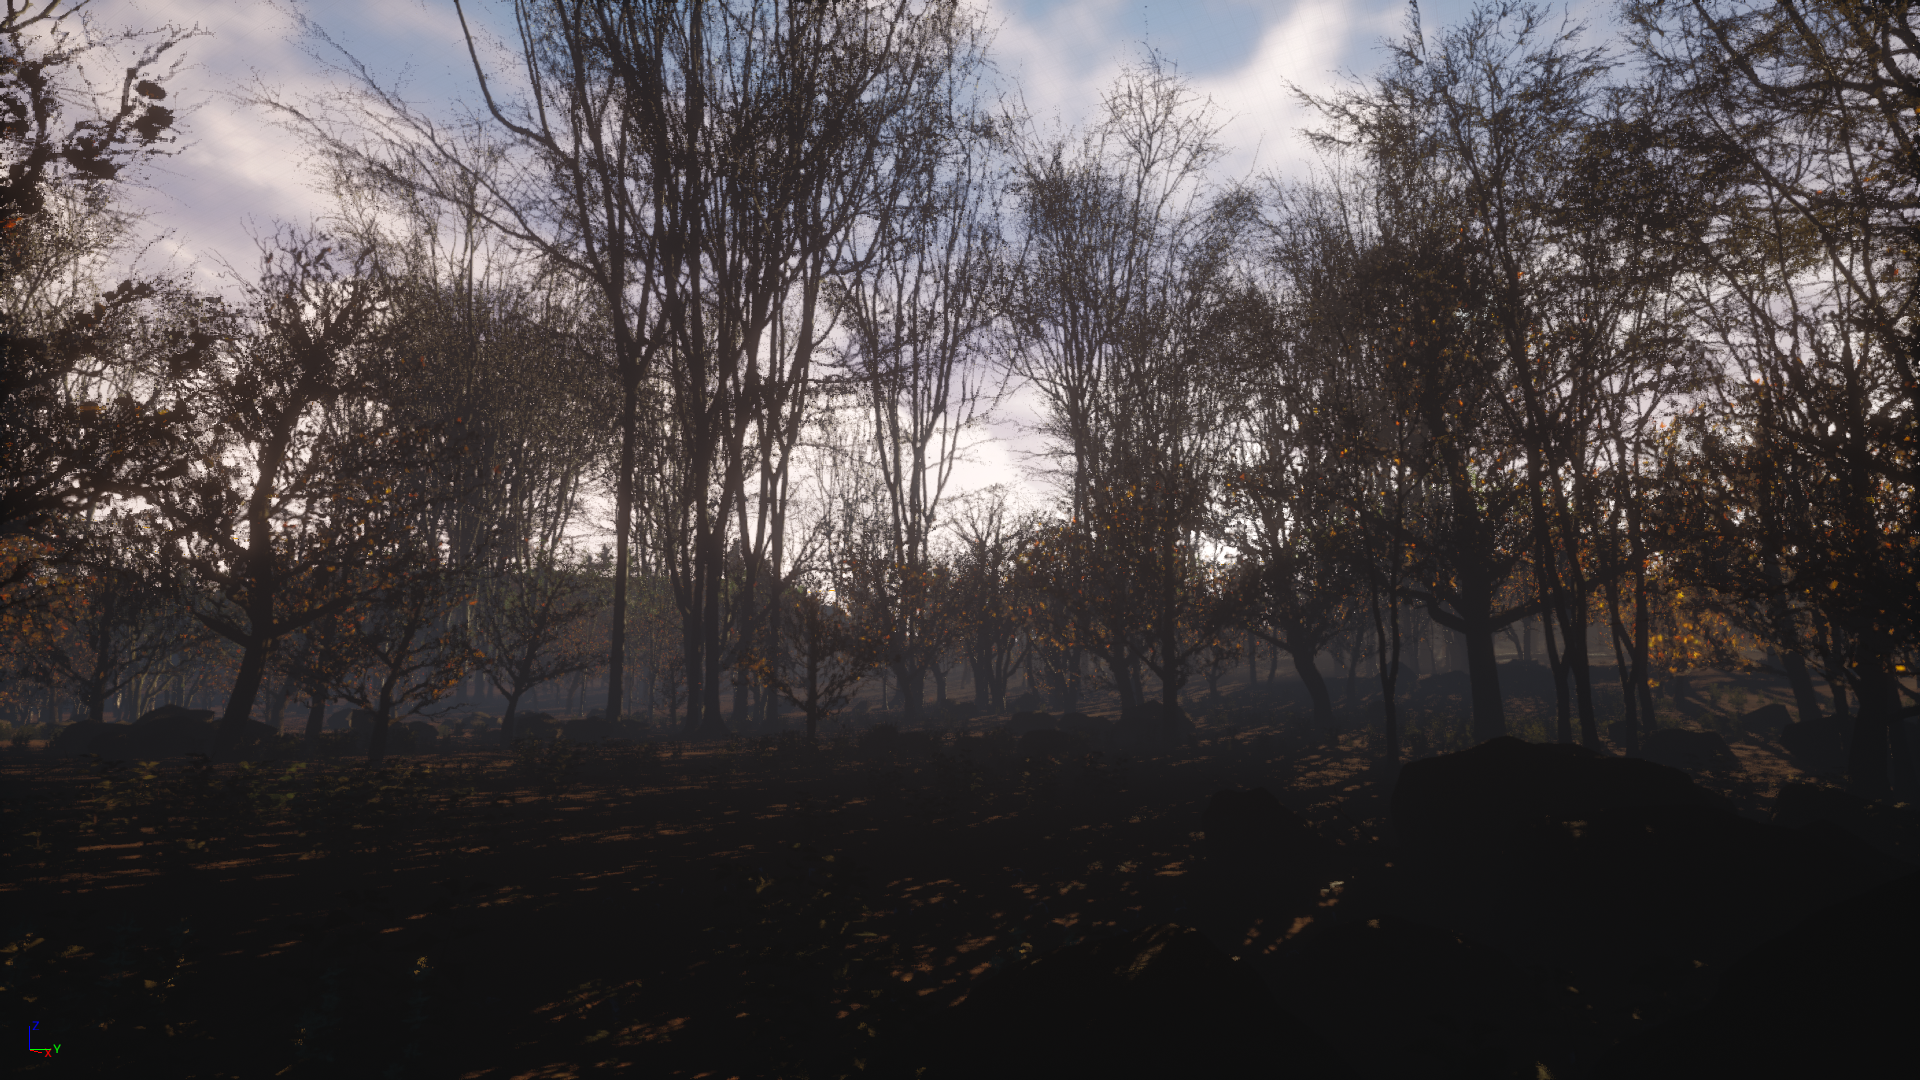
\includegraphics[width=\textwidth]{./img/screenshots/dayshot1.png}
  \end{center}
  \caption[ภาพฉากใน Two-player Cooperative Horror Game ตอนเย็น]{ภาพฉากใน Two-player Cooperative Horror Game ตอนเย็น}
  \label{fig:dayshot1}
\end{figure}

\begin{figure}[h]
  \begin{center}
  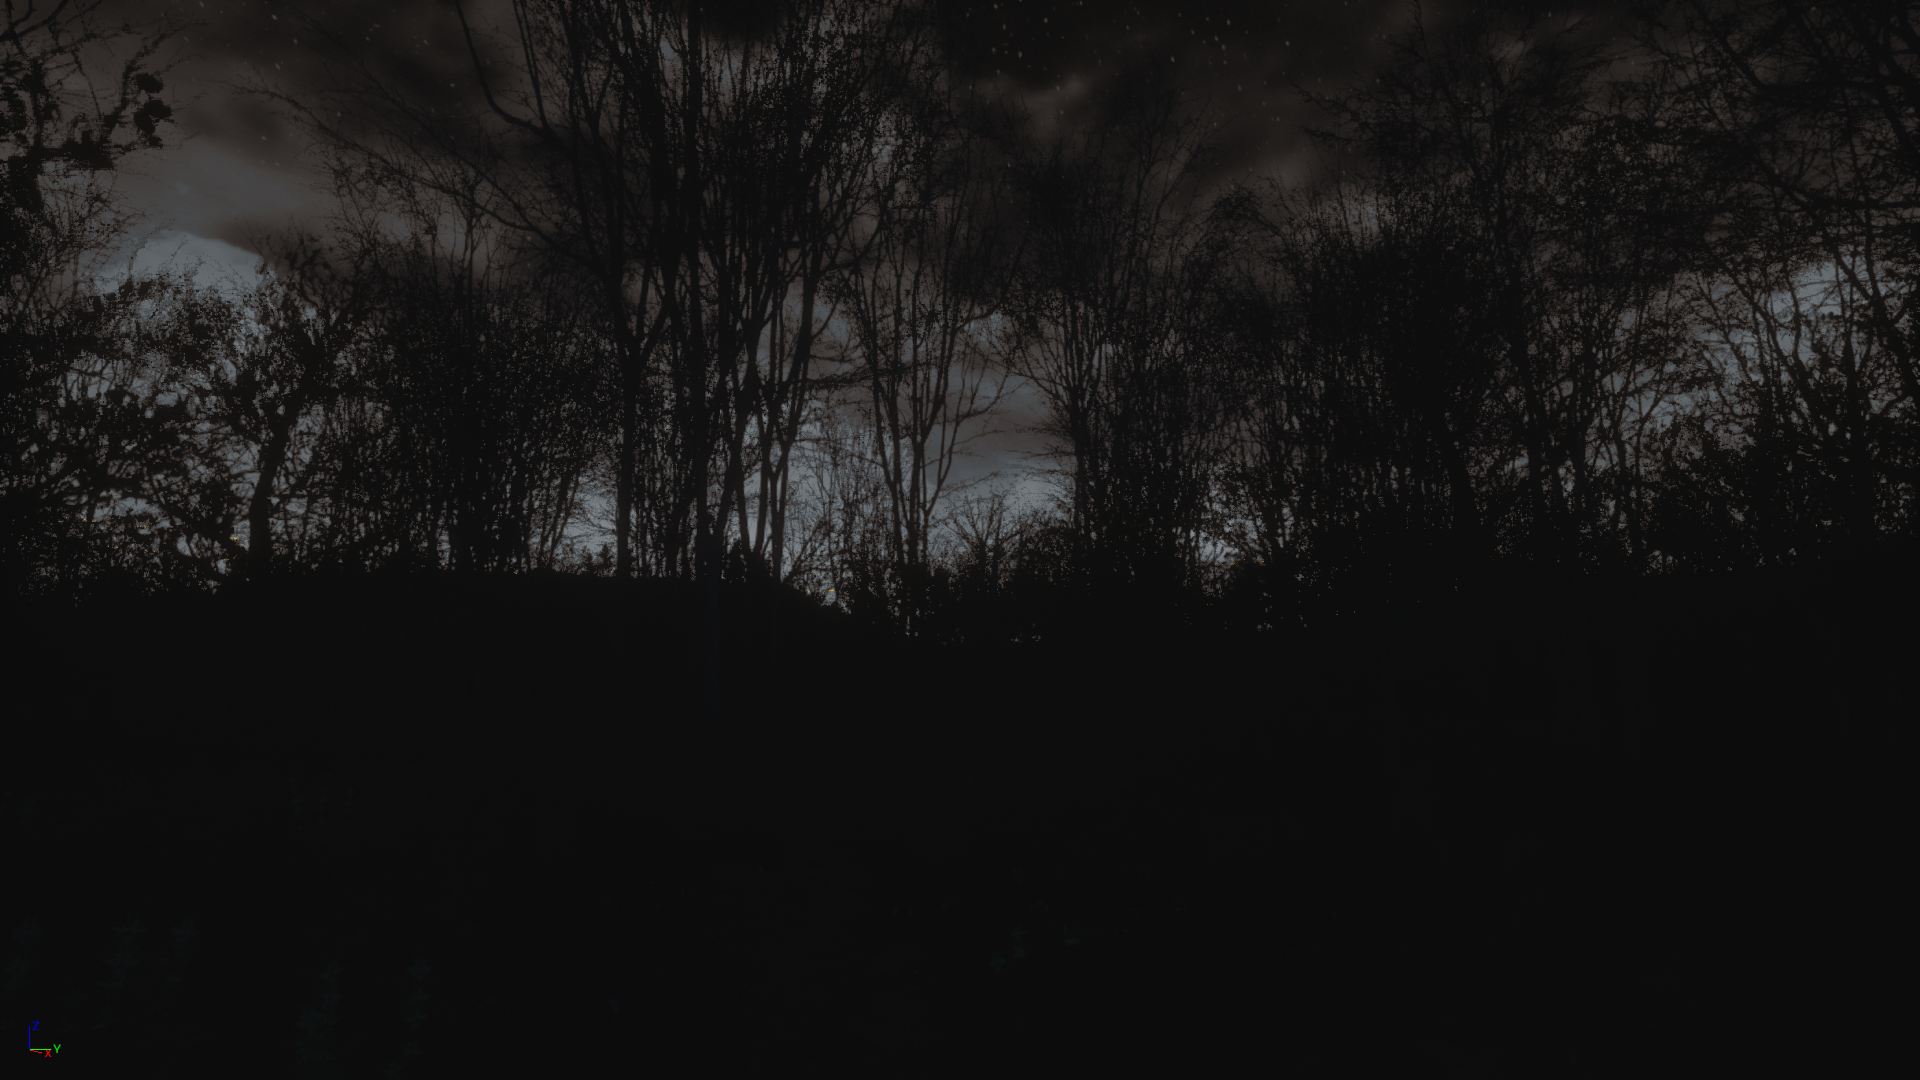
\includegraphics[width=\textwidth]{./img/screenshots/nightshot1.png}
  \end{center}
  \caption[ภาพฉากใน Two-player Cooperative Horror Game ตอนเย็น]{ภาพฉากใน Two-player Cooperative Horror Game ตอนกลางคืน}
  \label{fig:nightshot1}
\end{figure}

\subsection{การสิ้นสุดเกม}

\subsubsection{บริบท (Context)}

คุณสมบัตินี้จำเป็นต้องมีเพราะเป็นส่วนหนึ่งของ Game Loop

\subsubsection{สมมติฐาน (Hypothesis)}

การสิ้นสุดเกมโดยการทำลายวงแหวนเวทย์มนต์ให้ครบทุกวงทำได้เมื่อผู้เล่นวางแผนอย่างรอบคอบ สื่อสารกัน และทำงานร่วมมือกันได้ดี สัมพันธ์กับ Design Pillar ที่ 1

\subsubsection{วัดผลความสำเร็จ (Measuring success)}
ผู้เล่นสามารถจบเกมได้เมื่อวางแผนอย่างรอบคอบ สื่อสารกัน และทำงานร่วมมือกันได้ดี

\subsubsection{การออกแบบ (Design)}

ผู้เล่นสามารถเอาชนะปีศาจได้เมื่อทำลายวงแหวนเวทย์มนต์ได้ครบทุกอัน และจะแพ้เมื่อผู้เลนคนใดคนนึงเสียชีวิตหรือทั้งคู่ไม่สามารถทำลายวงแหวนเวทย์มนต์ในเวลาที่กำหนดได้

\subsection{การทำลายวงแหวนเวทย์มนต์}

\subsubsection{บริบท (Context)}

คุณสมบัตินี้จำเป็นต้องมีเพราะเป็นส่วนหนึ่งของ Game Loop

\subsubsection{สมมติฐาน (Hypothesis)}

การทำลายวงแหวนเวทย์มนต์ได้ผู้เล่นต้องมีชีวิตรอดจากปีศาจที่ตามจองล้างจองผลาญ และสามารถหาวงแหวนได้จากแผนที่และพลังวิเศษของแม่ชี สัมพันธ์กับ Design Pillar ที่ 1, 2

\subsubsection{วัดผลความสำเร็จ (Measuring success)}

ผู้เล่นสามารถเอาตัวรอดจากปีศาจได้และทำลายวงแหวนเวทย์มนต์ได้เมื่อหาเจอแล้ว

\subsubsection{การออกแบบ (Design)}

ผู้เล่นสามารถทำลายวงแหวนเวทย์มนต์โดยใช้ความสามารถพิเศษของแม่ชี การทำลายวงแหวนใช้เวลาไม่เกิน 1 นาที และจะเพิ่มความดุร้ายของปีศาจในรูปแบบของการเพิ่มความถี่ในการปรากฎตัว เพื่อให้เกิดความตึงเครียด และเพิ่มความเข้มข้น

\subsection{การเดินและการเคลื่อนไหวของตัวละคร}

\subsubsection{บริบท (Context)}

คุณสมบัติจำเป็นต้องมีเนื่องจากตัวละครต้องเคลื่อนไหวได้ในเกมอย่างสมจริง

\subsubsection{สมมติฐาน (Hypothesis)}
จำกัดการเคลื่อนไหวที่เป็นไปไม่ได้ในโลกจริงเพื่อเพิ่มความสมจริง การเคลื่อนไหวของปีศาจทำให้ผู้เล่นต้องเอาชีวิตรอด วางแผนทำภารกิจให้ดี การเคลื่อนไหวของ NPC ทำให้เกมสมจริงขึ้นเพิ่มความแนบเนียนให้กับปีศาจที่แฝงตัวอยู่ สัมพันธ์กับ Design Pillar ที่ 1, 3

\subsubsection{วัดผลความสำเร็จ (Measuring success)}

ผู้เล่นสามารถเอาชีวิตรอดได้เมื่อเคลื่อนไหวได้ด้วยความเร็วที่เหมาะสม และสามารถวางแผนทำภารกิจได้ด้วยความรอบคอบ ปีศาจโจมตีแบบลอบเร้นได้ดี มีความยาก ท้าทาย แต่ยังเล่นผ่านไปได้

\subsubsection{การออกแบบ (Design)}

\paragraph{การเคลื่อนไหวของผู้เล่น}

ผู้เล่นสามารถเคลื่อนที่ด้วยการเดิน กระโดด และวิ่ง โดยการวิ่งไม่สามารถวิ่งถอยหลังได้ สามารถวิ่งแล้วหันหน้ากลับมาดูข้างหลังเพียงชั่วคราวเท่านั้น

\paragraph{การเคลื่อนไหวของสัตว์}

สัตว์เดินและวิ่งด้วยความเร็วธรรมชาติของมันขึ้นอยู่กับชนิด จะอยู่กันเป็นฝูง ตัวปีศาจมีระบบ Navigation ที่ทำให้สามารถเคลื่อนที่ไปหาหรือติดตามผู้เล่นได้

\subsection{การต่อสู้}

\subsubsection{บริบท (Context)}
คุณสมบัตินี้จะเป็นการเล่นเกมในสถานการณ์ที่มีการโจมตีจากศัตรู และ การต่อสู้กับศัตรูเพื่อป้องกันตัวเอง 

\subsubsection{สมมติฐาน (Hypothesis)}
การที่ผู้เล่นสามารถต่อสู้ได้ จะทำให้ผู้เล่นวางแผนการ ต่อสู้กับศัตรูได้ และ การที่นายพรานสามารถต่อสู้ได้ แต่จะต้องใช้พลังในการต่อสู้มากกว่านายพราน จะทำให้ตัวเกมมีความสมดุลมากขึ้นโดยที่ตัวละครแต่ละตัวก็จะมีบทบาทในการเล่นเป็นของตัวเอง สัมพันธ์กับ Design Pillar ที่ 1, 2, 3

\subsubsection{วัดผลความสำเร็จ}
ผู้เล่นที่เล่นเป็นนายพรานสามารถต่อสู้กับศัตรูได้ และ ผู้เล่นที่เล่นเป็นแม่ชีสามารถต่อสู้กับศัตรูได้ โดยทำงานกันได้อย่างเป็นทีม

\subsubsection{การออกแบบ (Design)}

การต่อสู้สำหรับผู่เล่นมีไว้เพื่อป้องกันตัวเองจากการโจมตีของปีศาจเท่านั้น ไม่ได้มีไว้เพื่อฆ่าปีศาจ ผู้ที่เล่นเป็นแม่ชีเท่านั้นที่สามารถป้องกันการโจมตีของปีศาจได้ โดยหลังจากผู้เล่นป้องกันการโจมตี เขาจะบาดเจ็บ เสีย HP ผู้เล่นสามารถป้องกันการโจมตีได้เรื่อย ๆ จนกว่าจะตาย โดยปีศาจจะโจมตีทีละครั้งเท่านั้น ความถี่ในการโจมตีขึ้นอยู่กับจำนวนวงแหวนเวทย์มนต์ที่ผู้เล่นได้ทำลายไป

การโจมตีของปีศาจ ปีศาจจะเข้าหาผู้เล่นแบบลอบเร้น (Stealth) และจะโจมตีโดยการปล่อยพลังเวทย์ เสียงดนตรีและเสียงประกอบจะดังขึ้นตอนนี้ ผู้เล่นสามารถป้องกันการโจมตีได้ ถ้าหากป้องกันได้ก่อนที่ปีศาจจะโจมตี จะไม่ได้รับ Damage แต่ถ้าเริ่มโจมตีแล้วจะลด Damage เพียงกึ่งหนึ่ง

\subsection{การรักษา}

\subsubsection{บริบท (Context)}

คุณสมบัตินี้จำเป็นต้องมีเพื่อให้ผู้เล่นรักษาตัวเองได้หลังจากถูกโจมตี

\subsubsection{สมมติฐาน (Hypothesis)}

การที่นายพรานสามารถรักษาได้จะทำให้ตัวเกมมีความสมดุลมากขึ้นโดยที่ตัวละครแต่ละตัวก็จะมีบทบาทในการเล่นเป็นของตัวเอง เพื่อภาระหน้าที่ในการทำงานกันเป็นทีม สัมพันธ์กับ Design Pillar ที่ 1, 2, 3

\subsubsection{วัดผลความสำเร็จ}

ผู้เล่นที่เล่นเป็นนายพราน สามารถรักษาตัวเองได้ และผู้เล่นที่เล่นเป็นแม่ชีไม่สามารถรักษาตัวเองได้ สามารถทำงานกันได้อย่างเป็นทีมเพื่อทำภารกิจได้

\subsubsection{การออกแบบ (Design)}

ผู้เล่นที่เล่นเป็นนายพรานสามารถรักษาตัวเองได้ แต่ผู้เล่นที่เล่นเป็นแม่ชีไม่สามารถรักษาตัวเองได้
นายพรานต้องเก็บสมุนไพรในป่าเพื่อนำมารักษา

\subsection{กับดัก}

\subsubsection{บริบท (Context)}

คุณสมบัตินี้ จะใช้เมื่อผู้เล่นต้องการปลดกับดัก ผู้เล่นที่เล่นเป็นนายพรานสามารถปลดกับดักได้ แต่ผู้เล่นที่เล่นเป็นแม่ชีไม่สามารถปลดกับดักได้ เพื่อให้ผู้เล่นมีความระแวดระวังอยู่ตลอดเวลา

\subsubsection{สมมติฐาน (Hypothesis)}

เพิ่มความท้าทายให้กับผู้เล่นและการที่นายพรานสามารถปลดกับดักได้จะทำให้ตัวเกมมีความสมดุลมากขึ้น \\ โดยที่ตัวละครแต่ละตัวก็จะมีบทบาทในการเล่นเป็นของตัวเอง สัมพันธ์กับ Design Pillar ที่ 1, 2, 3

\subsubsection{วัดผลความสำเร็จ}

ผู้เล่นที่เล่นเป็นนายพราน สามารถปลดกับดักได้ และผู้เล่นที่เล่นเป็นแม่ชีไม่สามารถปลดกับดักได้ โดยทำงานกันได้อย่างเป็นทีม มีความระแวดระวัง และสื่อสารกันได้ดี

\subsubsection{การออกแบบ (Design)}

กับดักในป่าสามารถทำให้แม่ชีบาดเจ็บได้เพียงแค่เดินเหยียบ ผู้ที่เล่นเป็นนายพรานสามารถมองเห็นและปลดกับดักได้ นายพรายไม่สามารถถูกกับดักทำร้ายได้

\subsubsection{วัดผลความสำเร็จ}

ผู้เล่นที่เล่นเป็นนายพราน สามารถรักษาตัวเองได้ และผู้เล่นที่เล่นเป็นแม่ชีไม่สามารถรักษาตัวเองได้ สามารถทำงานกันได้อย่างเป็นทีมเพื่อทำภารกิจได้

\subsubsection{การออกแบบ (Design)}

ผู้เล่นที่เล่นเป็นนายพรานสามารถรักษาตัวเองได้ แต่ผู้เล่นที่เล่นเป็นแม่ชีไม่สามารถรักษาตัวเองได้
นายพรานต้องเก็บสมุนไพรในป่าเพื่อนำมารักษา

\subsection{แผนที่นำทาง}

\subsubsection{บริบท (Context)}
คุณสมบัติในการใช้แผนที่เป็นหนึ่งในสิ่งที่ทำให้ผู้เล่นใช้ในการวางแผนการเล่นเกม ผู้เล่นที่รับบทเป็นนายพรานจะเป็นผู้ถือแผนที่


\subsubsection{สมมติฐาน (Hypothesis)}
ทำให้ผู้เล่นได้วางแผนการเล่นอย่างรอบ เพื่อที่จะชนะเกม  สัมพันธ์กับ Design Pillar ที่ 1, 2, 3

\subsubsection{วัดผลความสำเร็จ}
ผู้เล่นที่เล่นเป็นนายพราน สามารถวางแผนการเล่นได้ และผู้เล่นที่เล่นเป็นแม่ชีไม่สามารถวางแผนการเล่นได้ โดยทำงานกันได้อย่างเป็นทีม มีความระแวดระวัง และสื่อสารกันได้ดี ผู้เล่นวางแผนการเล่นได้ง่ายขึ้น ไม่หลงทาง

\subsubsection{การออกแบบ (Design)}

นายพรานเป็นผู้ชำนาญการในป่า เขามีหน้าที่นำทางโดยใช้แผนที่ เมื่อเดินไปที่ไหนแผนที่จากที่เรือนรางจะปรากฏขึ้น แสดงลักษณะภูมิประเทศ คล้ายตัวอย่างจากเกม Minecraft ในรูป \ref{fig:minecrafmap-blank}, \ref{fig:minecrafmap-partial} นายพรานสามารถทำสัญลักษณ์บนแผนที่เพื่อแสดงจุดที่สนใจ นายพรานจะควักแผนที่ออกมา ใช้แผนที่ที่อยู่ตรงหน้าเขาในการ \\ นำทาง ดังตัวอย่างจากเกม Metro Exodus ในรูป \ref{fig:metromap}

\begin{figure}[h]
  \begin{center}
  
\includegraphics[width=\textwidth]{./img/minecraftmap-blank.png}
  \end{center}
  \caption[ตัวอย่างกลไกของแผนที่เมื่อผู้เล่นยังไม่ได้ทำการสำรวจจากเกม Minecraft]{ตัวอย่างกลไกของแผนที่เมื่อผู้เล่นยังไม่ได้ทำการสำรวจจากเกม Minecraft แสดงแผนที่ที่ว่างเปล่า}
  \label{fig:minecrafmap-blank}
\end{figure}


\begin{figure}[h]
  \begin{center}
  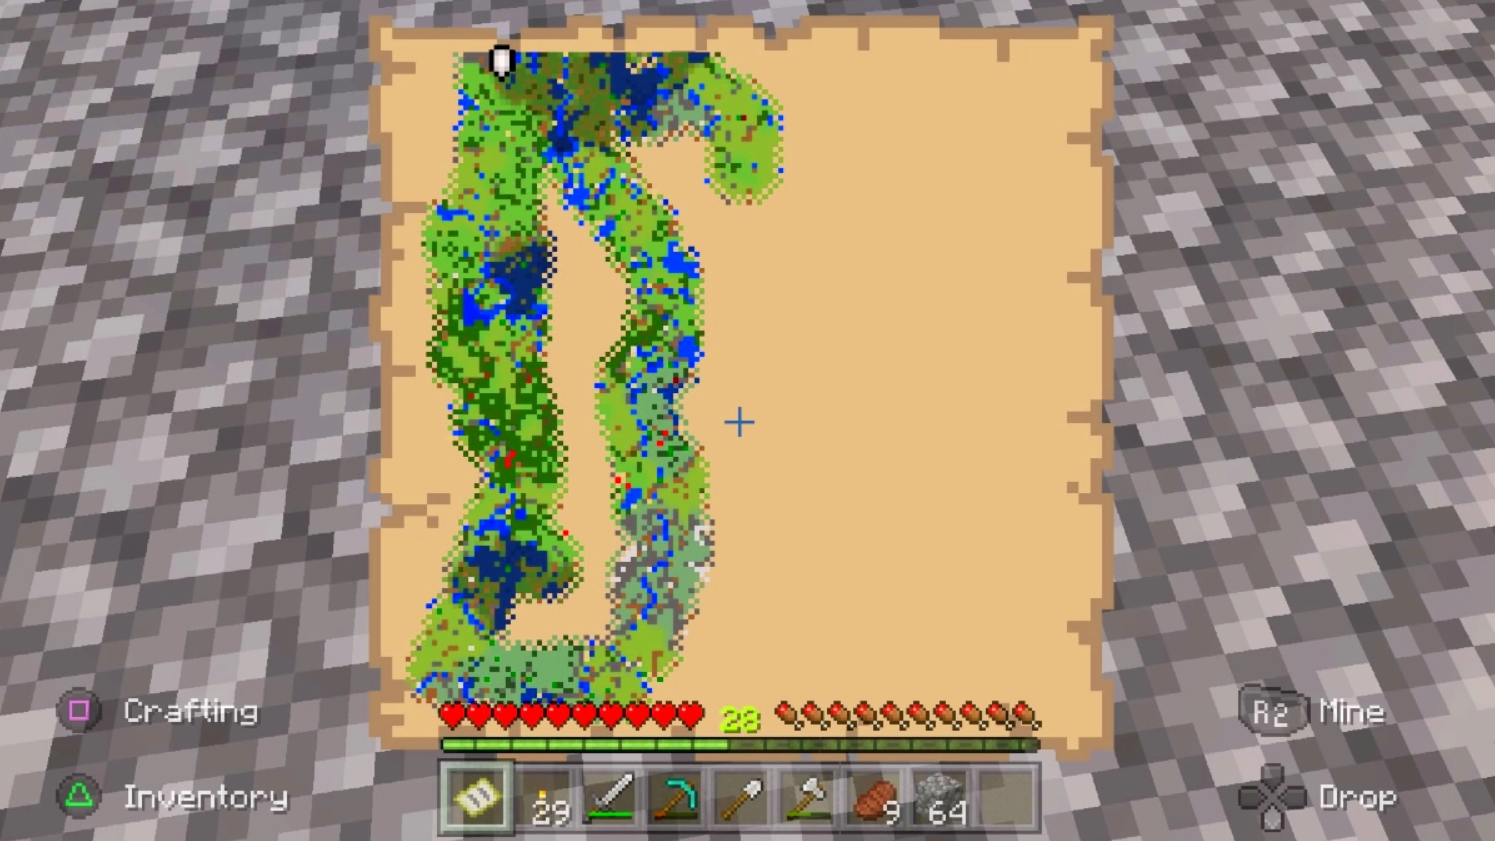
\includegraphics[width=\textwidth]{./img/minecraftmap-partial.png}
  \end{center}
  \caption[ตัวอย่างกลไกของแผนที่เมื่อผู้เล่นทำการสำรวจแล้วบางส่วน จากเกม Minecraft]{ตัวอย่างกลไกของแผนที่เมื่อผู้เล่นทำการสำรวจแล้วบางส่วน จากเกม Minecraft แสดงแผนที่ที่ปรากฏภูมิประเทศแล้วบางส่วน}
  \label{fig:minecrafmap-partial}
\end{figure}

\begin{figure}[h]
  \begin{center}
  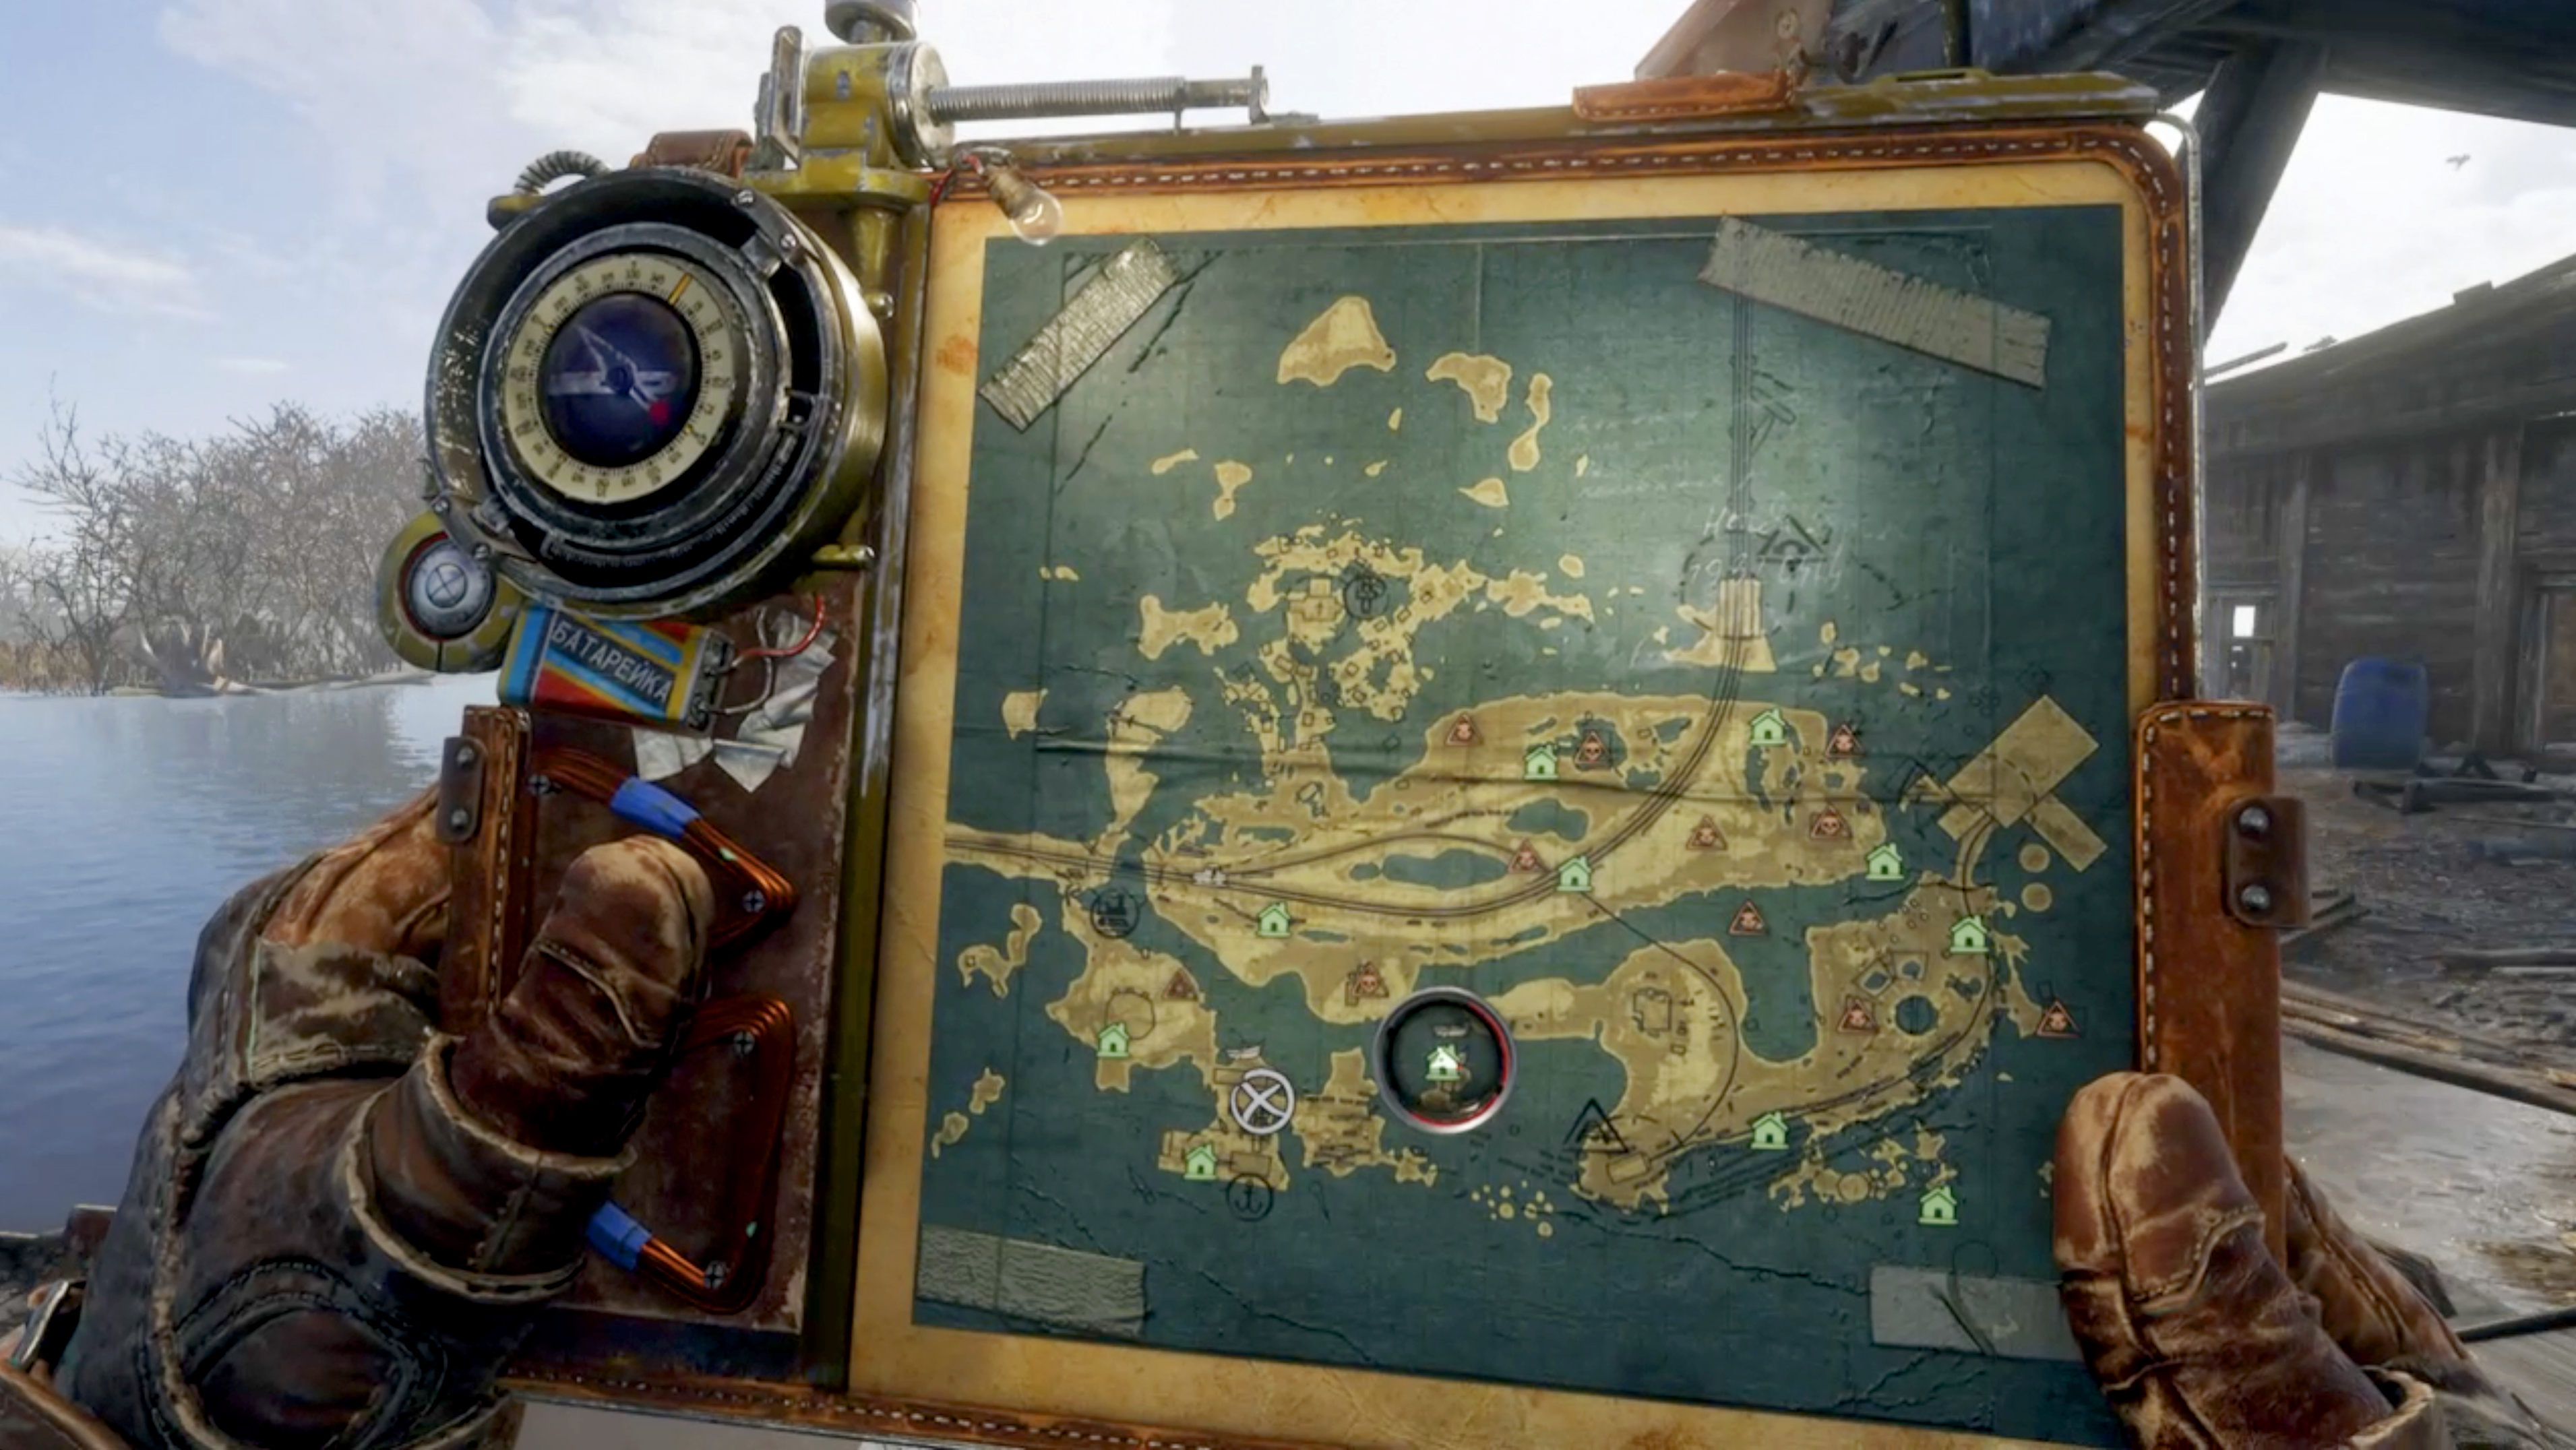
\includegraphics[width=\textwidth]{./img/metromap.jpg}
  \end{center}
  \caption[ตัวอย่างกลไกการใช้แผนที่ของเกม Metro Exodus]{ตัวอย่างกลไกการใช้แผนที่ของเกม Metro Exodus ตัวละครควักแผนที่ออกมาจากกระเป๋า เสมือนว่าเขากำลังถือแผนที่อยู่ตรงหน้าจริง ๆ}
  \label{fig:metromap}
\end{figure}